\documentclass[a4paper,12pt,oneside]{book}

%-------------------------------Start of the Preable------------------------------------------------
\usepackage[english]{babel}
\usepackage{blindtext}
%packagr for hyperlinks
\usepackage{hyperref}
\hypersetup{
    colorlinks=true,
    linkcolor=blue,
    filecolor=magenta,
    urlcolor=cyan,
}

\urlstyle{same}
%use of package fancy header
\usepackage{fancyhdr}
\setlength\headheight{26pt}
\fancyhf{}
%\rhead{
\includegraphics[width=1cm]{logo}}
\lhead{\rightmark}
\rhead{
\includegraphics[width=1cm]{logo}}
\fancyfoot[RE, RO]{\thepage}
\fancyfoot[CE,CO]{\href{http://www.e-yantra.org}{www.e-yantra.org}}

\pagestyle{fancy}

%use of package for section title formatting
\usepackage{titlesec}
\titleformat{\chapter}
  {\Large\bfseries} % format
  {}                % label
  {0pt}             % sep
  {\huge}           % before-code

%use of package tcolorbox for colorful textbox
\usepackage[most]{tcolorbox}
\tcbset{colback=cyan!5!white,colframe=cyan!75!black,halign title = flush center}

\newtcolorbox{mybox}[1]{colback=cyan!5!white,
colframe=cyan!75!black,fonttitle=\bfseries,
title=\textbf{\Large{#1}}}

%use of package marginnote for notes in margin
\usepackage{marginnote}

%use of packgage watermark for pages
%\usepackage{draftwatermark}
%\SetWatermarkText{
\includegraphics{logo}}
\usepackage[scale=2,opacity=0.1,angle=0]{background}
\backgroundsetup{
contents={
\includegraphics{logo}}
}

%use of newcommand for keywords color
\usepackage{xcolor}
\newcommand{\keyword}[1]{\textcolor{red}{\textbf{#1}}}

%package for inserting pictures
\usepackage{graphicx}

%package for highlighting
\usepackage{color,soul}

%new command for table
\newcommand{\head}[1]{\textnormal{\textbf{#1}}}


%----------------------End of the Preamble---------------------------------------


\begin{document}

%---------------------Title Page------------------------------------------------
\begin{titlepage}
\raggedright
{\Large eYSIP2016\\[1cm]}
{\Huge\scshape Robot State Collector\\[.1in]}
\vfill
\begin{flushright}
{\large Amanpreet Singh \\}
{\large Amit Raushan \\}
{\large Shubham Gupta \\}
{\large Duration of Internship: $ 10/06/2016-24/07/2016 $ \\}
\end{flushright}

{\itshape 2016, e-Yantra Publication}

\end{titlepage}

\tableofcontents

%------------------------------------------------------------------------

\chapter[Robot State Collector]{Robot State Collector}
\section{Abstract}

\hspace{5mm}This project aims at developing a State Collection Code which is easy to merge with any code and doesn't interfere with the code already present in the Robot. Our code should be capable of sending the sensor values collected periodically to the GUI developed for this specific purpose which would be able to encrypt the collected data and send it to the e-Yantra servers.

This would be helpful in re-creating runs ,using the code and the data collected by us, virtually.

The main tasks involved in the project are :

\begin{enumerate}

    \item Collecting timed data about the state of the robot(sensors etc.).
    \item Finding a way to efficiently storing data on the robot for a single run of the robot.
    \item Developing a GUI that picks up the data from the robot,encrypts it and send it to e-yantra servers.

\end{enumerate}
\newpage

\section{Completion status}

\begin{enumerate}

    \item We have been able to collect the data on Firebird V after a particular time period (currently set as 0.5s).
    \item To avoid storing the data on the volatile memory on any robot we are using a X-Bee module which directly sends the data to the GUI wirelessly and by doing so we even save space on the robot's memory.
    \item We have developed a GUI to read the incoming data from the Robot , encrypt the data and send it back to the server. The GUI is also capable of detecting is any changes were made to the file before sending it to the server.
    \item We have also made a Robot using the TIVA board so as to check that our code and GUI are not restricted to only Firebird V.
    \item We have been able to perform state collection on the newly developed robot.
\newpage

\end{enumerate}

\section{Hardware parts used}

\begin{itemize}
  \item Hardware used with FireBird V :
  \\
  \begin{figure}[h]
        \centering
        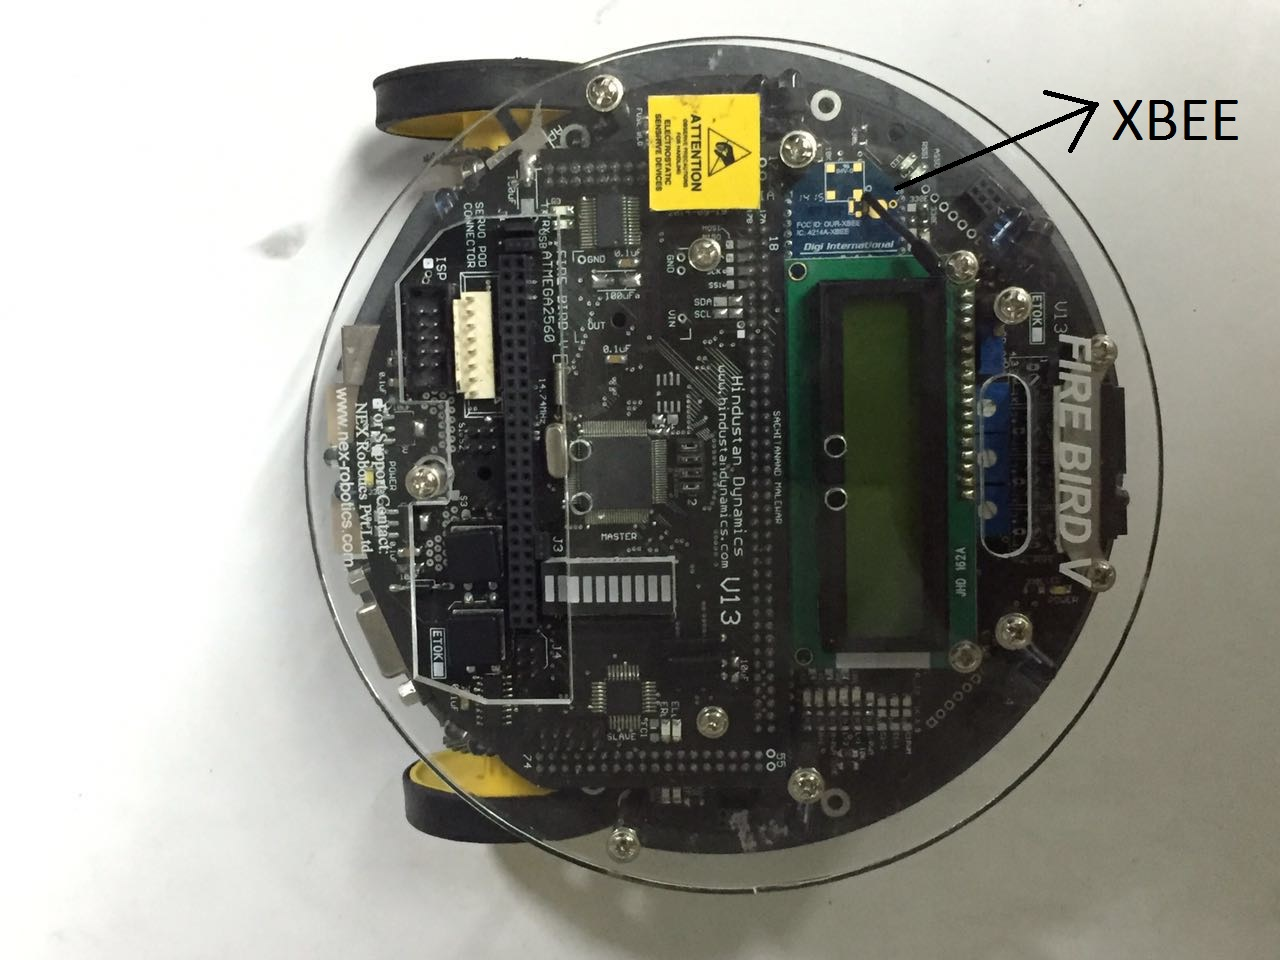
\includegraphics[scale=0.2]{firebird_V}
        \caption{Firebird V with Xbee module}
      \end{figure}

  \begin{enumerate}
    \item X-Bee Module.\\
    \href{https://www.sparkfun.com/datasheets/Wireless/Zigbee/XBee-Datasheet.pdf}{ Datasheet}
    \begin{figure}[h]
        \centering
        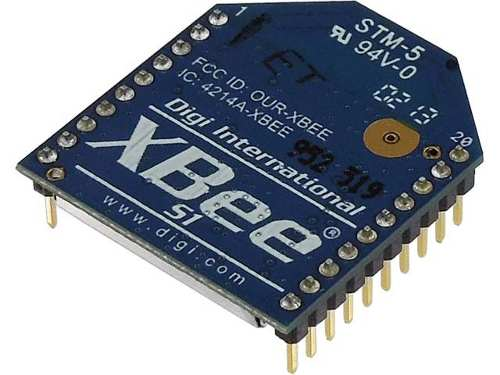
\includegraphics[scale=0.35]{xbee.jpg}
        \caption{xbee module}
      \end{figure}
      \newpage
    \item X-Bee Module and adapter to receive data on a Laptop/PC.\par

    \begin{figure}[!ht]
        \centering
        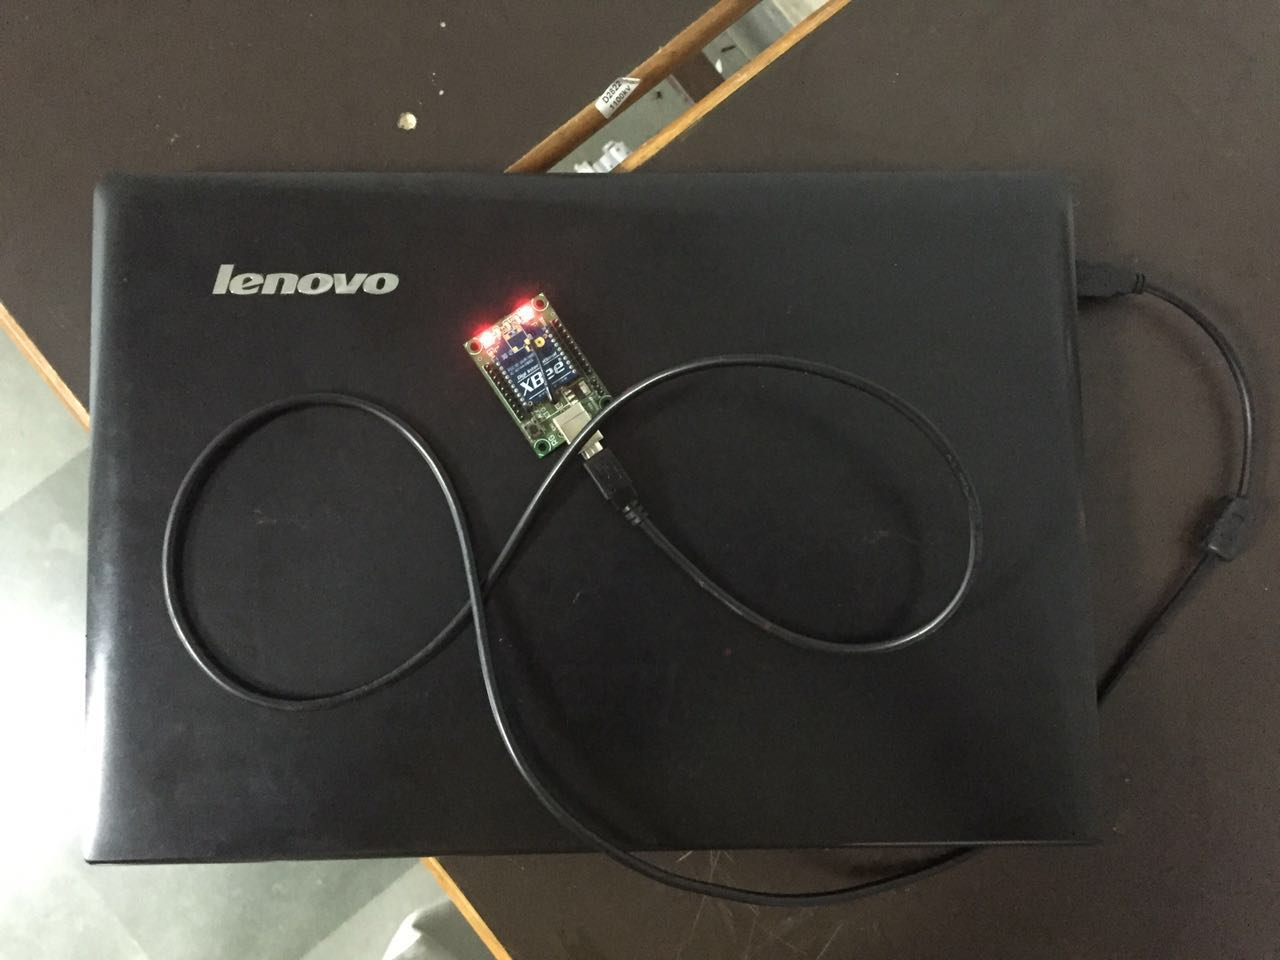
\includegraphics[scale=0.15]{adapter_board}
        \caption{Xbee with adapter connected to laptop}
      \end{figure}
  \end{enumerate}

  \item Hardware used to build a Robot using TIVA board (TM4C123GXL)\\
  \href{http://www.ti.com.cn/cn/lit/ds/symlink/tm4c123gh6pm.pdf}{ Datasheet}\\
  \href{http://www.ti.com/lit/ug/spmu298a/spmu298a.pdff}{ Pheripheral Driver Library}\\
  \href{http://www.mouser.com/ds/2/405/spmu296-242111.pdf}{User's Guide}
  \begin{figure}[h]
        \centering
        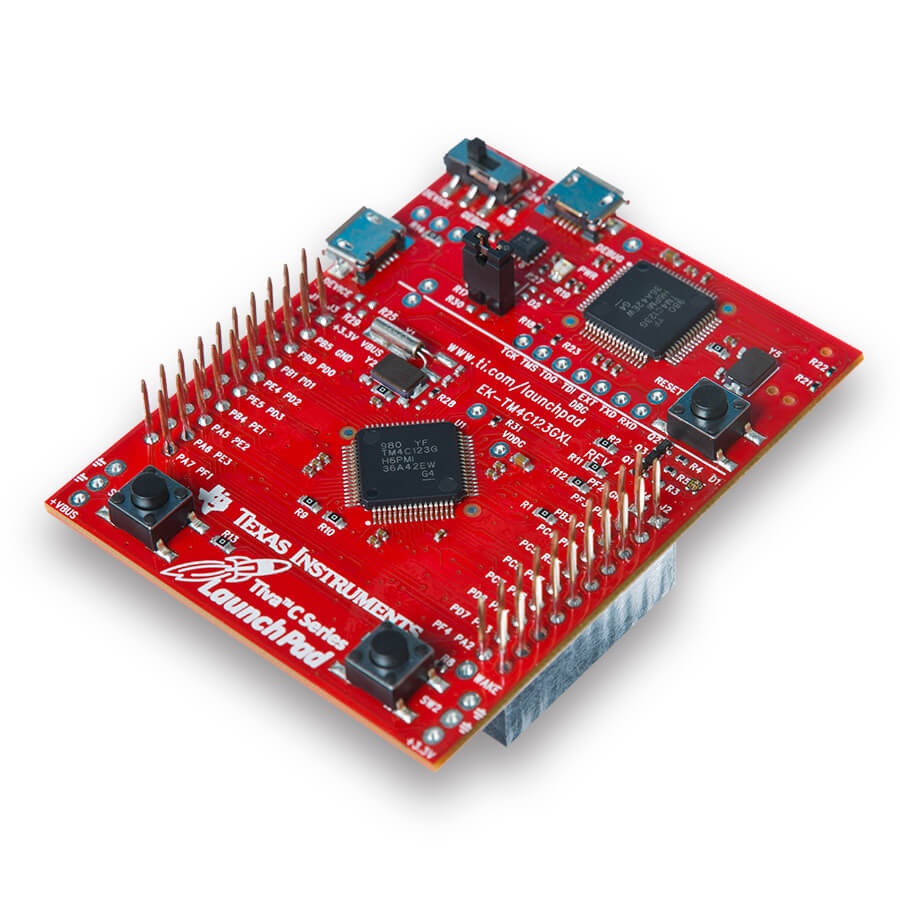
\includegraphics[scale=0.2]{tiva}
        \caption{Tiva C Series TM4C123G LaunchPad}
      \end{figure}
       \newpage
  \begin{enumerate}
   \item 2x DG02S Mini DC Gear motor.\\
   \href{http://cdn.sparkfun.com/datasheets/Robotics/DG02S.pdf}{ Datasheet}
   \begin{figure}[!ht]
        \centering
        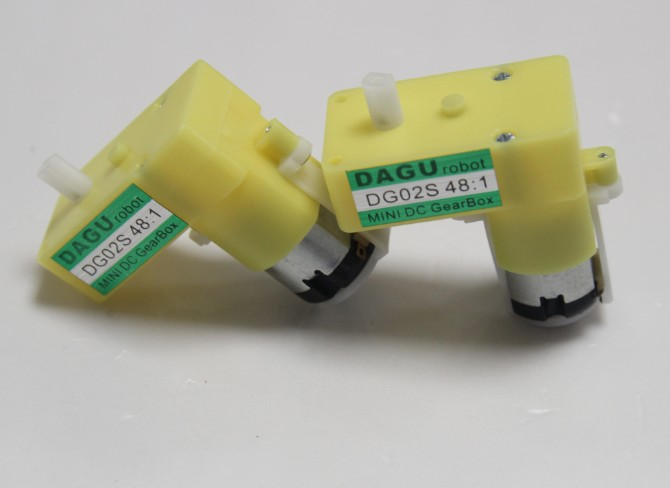
\includegraphics[scale=0.25]{motor}
        \caption{DC Geared motor}
      \end{figure}

    \item 2x Wheel - 65mm.
    \begin{figure}[h]
        \centering
        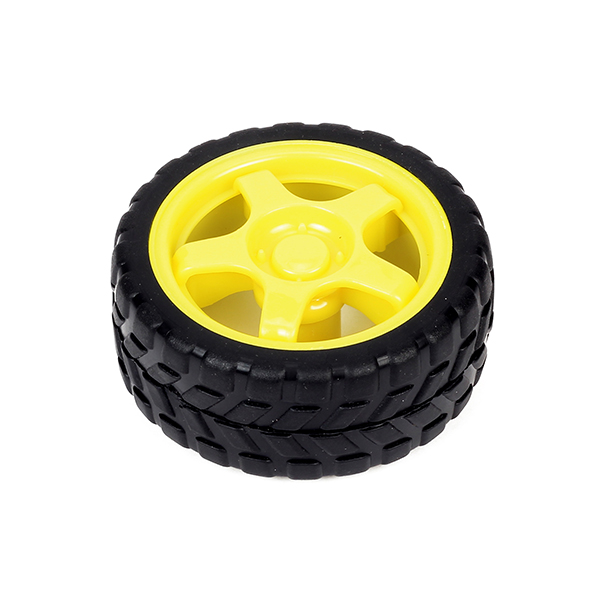
\includegraphics[scale=0.22]{wheel}
        \caption{Wheel}
      \end{figure}
    \item L293D - Motor Driver.\\
    \href{http://www.engineersgarage.com/sites/default/files/L293D.pdf}{ Datasheet}\par
   \begin{figure}[!ht]
        \centering
        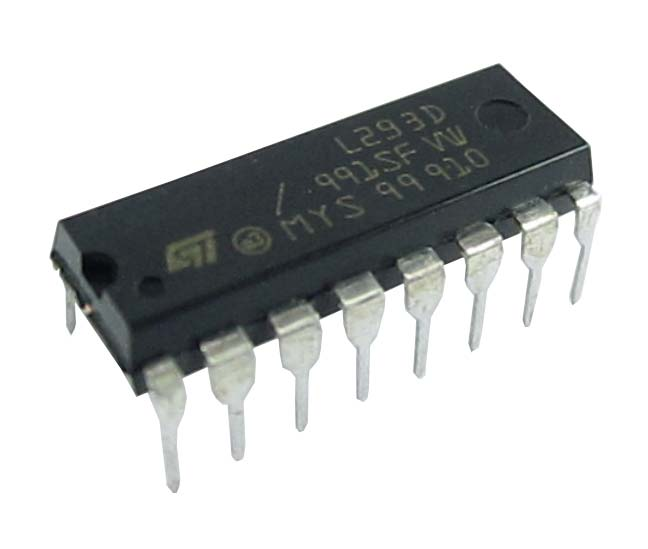
\includegraphics[scale=0.2]{l293d}
        \caption{Motor Driver IC}
      \end{figure}
      \newpage
    \item 16x2 LCD.\\
    \href{http://www.engineersgarage.com/sites/default/files/LCD\%2016x2.pdf}{ Datasheet}\par
   \begin{figure}[!ht]
        \centering
        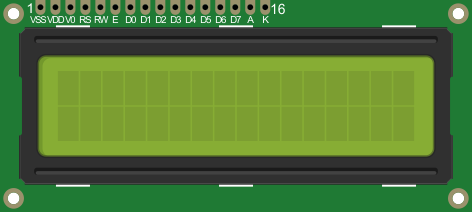
\includegraphics[scale=0.85]{lcd}
        \caption{LCD 16x2 Display}
      \end{figure}
    \item White Line Sensor Module.\\
    \href{http://www.nex-robotics.com/images/downloads/3\%20channel\%20line\%20sensor.pdf}{ Manual}\par
   \begin{figure}[!ht]
        \centering
        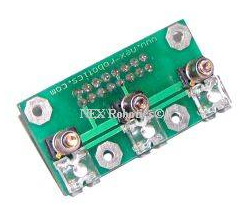
\includegraphics[scale=0.85]{whiteline}
        \caption{3 Channel Whiteline Sensors}
      \end{figure}
    \item SHARP 0A41SK sensor.\\
    \href{http://www.sharp-world.com/products/device/lineup/data/pdf/datasheet/gp2y0a41sk_e.pdf}{ Datasheet}\par
   \begin{figure}[!ht]
        \centering
        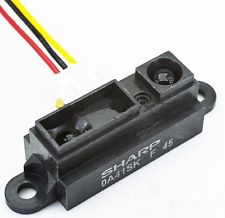
\includegraphics[scale=0.8]{sharp}
        \caption{SHARP Sensor}
      \end{figure}
    \item Caster Wheel.
    \begin{figure}[!ht]
        \centering
        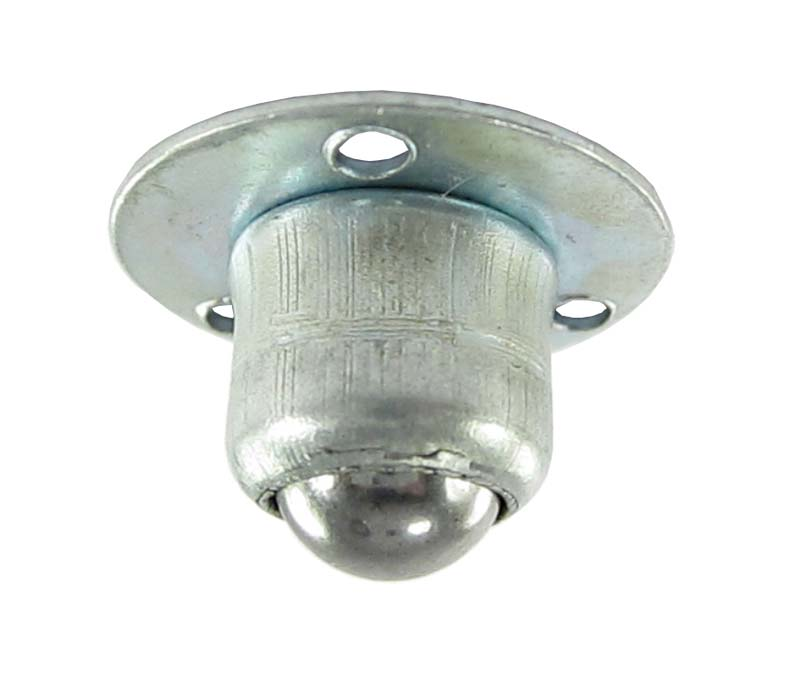
\includegraphics[scale=0.15]{caster}
        \caption{Caster Wheel}
      \end{figure}
    \item LM3237 - Voltage Regulator.\\
    \href{http://pdf.datasheetarchive.com/indexerfiles/Datasheet-044/DSA0017815.pdf}{ Datasheet}\par
   \begin{figure}[!ht]
        \centering
        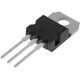
\includegraphics[scale=1]{lm}
        \caption{LM3237}
      \end{figure}
    \item Heat Sink.
    \begin{figure}[!ht]
        \centering
        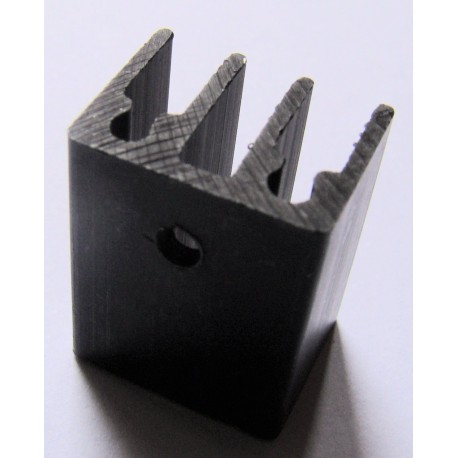
\includegraphics[scale=0.25]{heat}
        \caption{Heat Sink}
      \end{figure}
      \newpage
    \item 10 micro farad Electrolyte Capacitor.
    \begin{figure}[!ht]
        \centering
        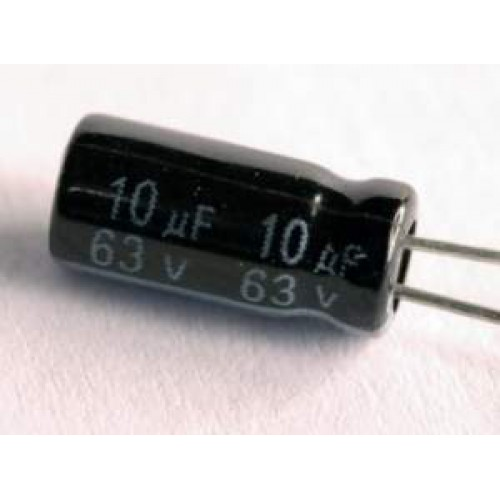
\includegraphics[scale=0.35]{cap}
        \caption{Capacitor}
      \end{figure}
    \item Multi-purpose PCB board. \\
    \begin{figure}[!h]
        \centering
        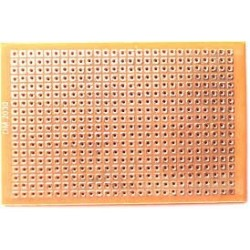
\includegraphics[scale=0.6]{pcb}
        \caption{PCB Board}
      \end{figure}
    \item 12V Rechargeable Battery.
    \begin{figure}[!h]
        \centering
        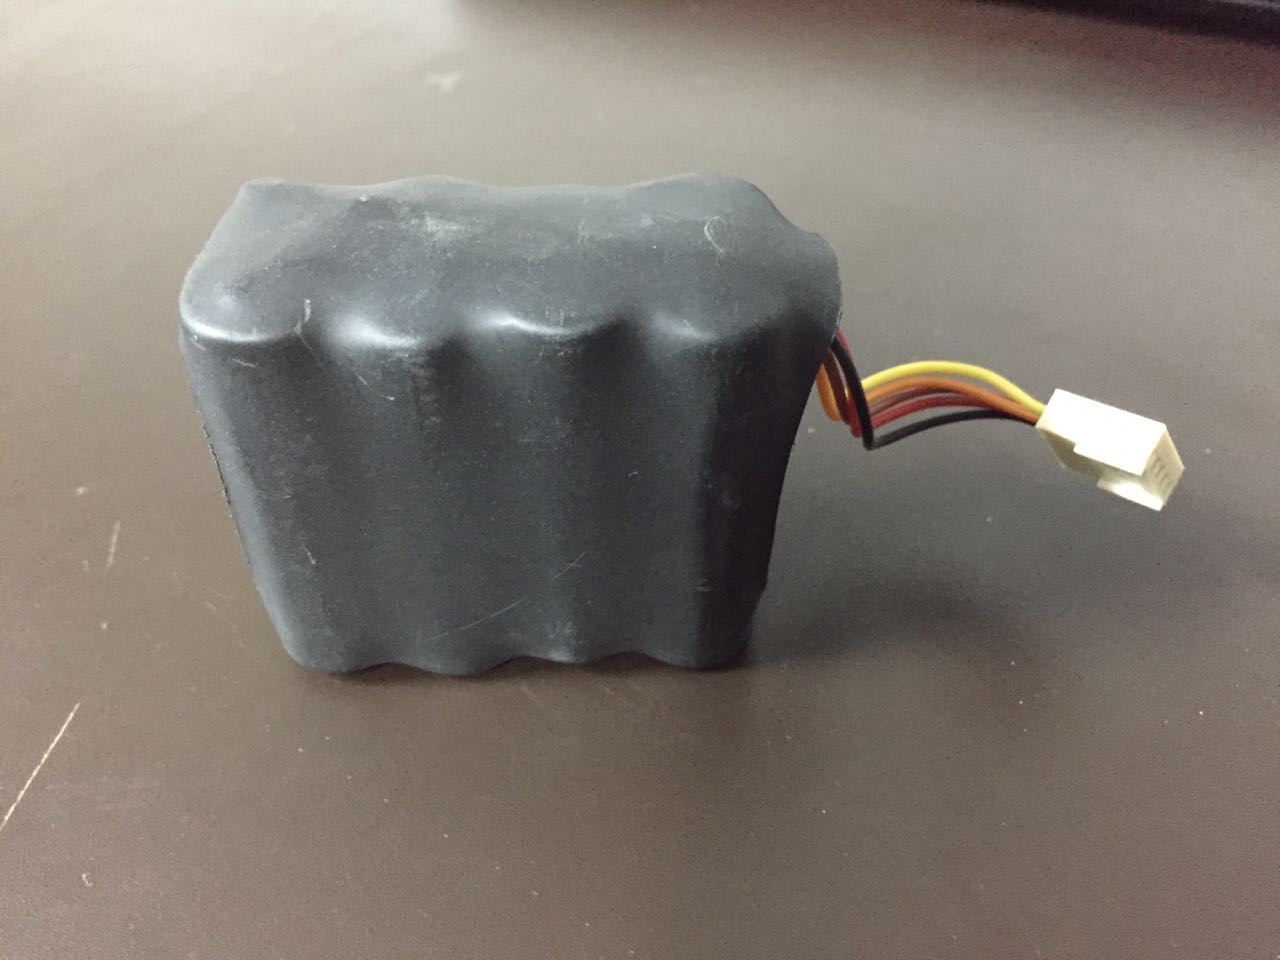
\includegraphics[scale=0.12]{battery}
        \caption{12V Rechargeable Battery}
      \end{figure}
      \newpage
    \item 20 Pin Planar Cable.
    \begin{figure}[!h]
        \centering
        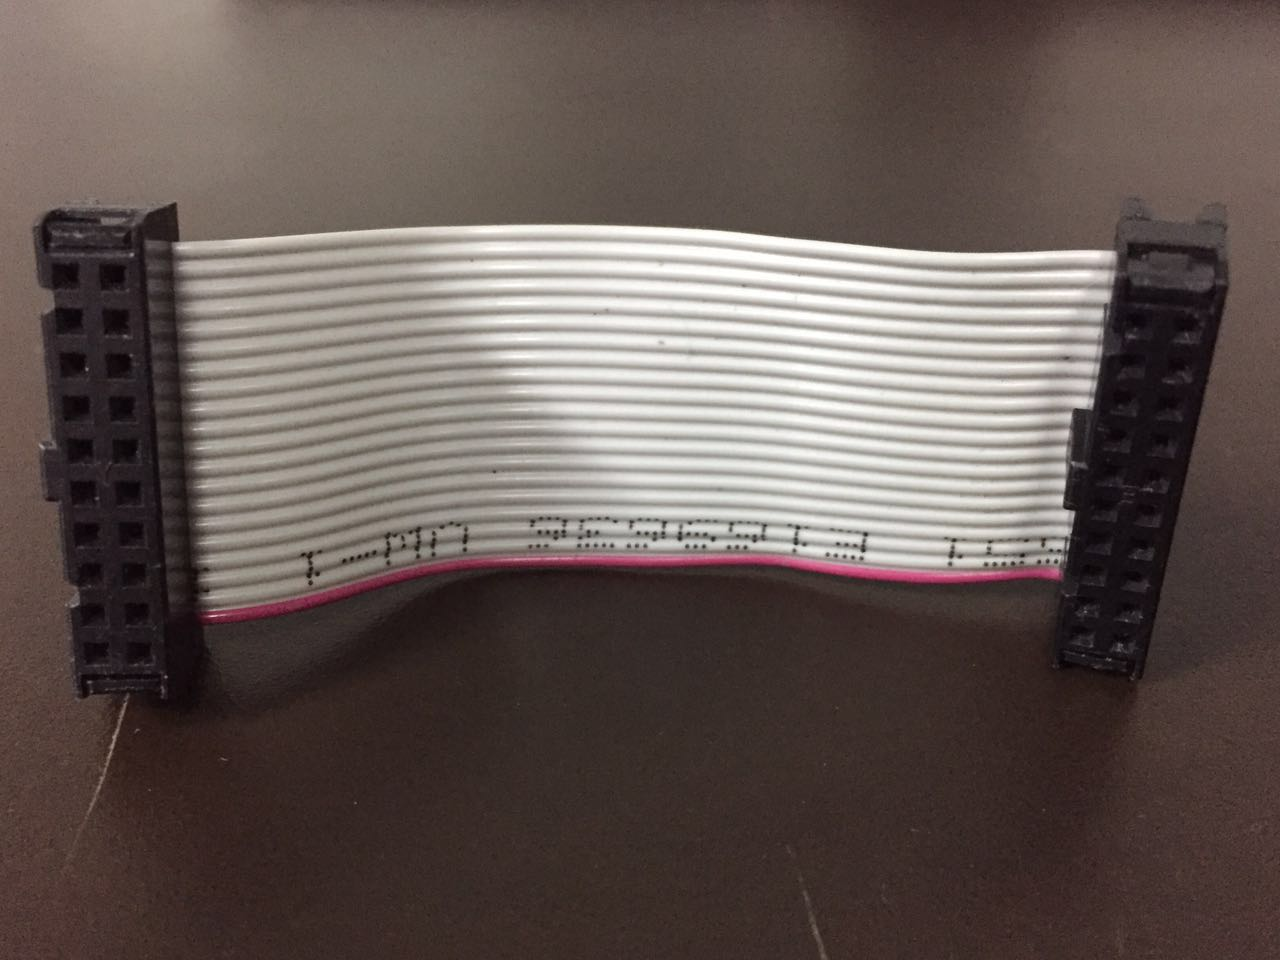
\includegraphics[scale=0.1]{wire}
        \caption{20 pin Connector wire}
      \end{figure}
    \item Female bug strip.
    \\
    \begin{figure}[!h]
        \centering
        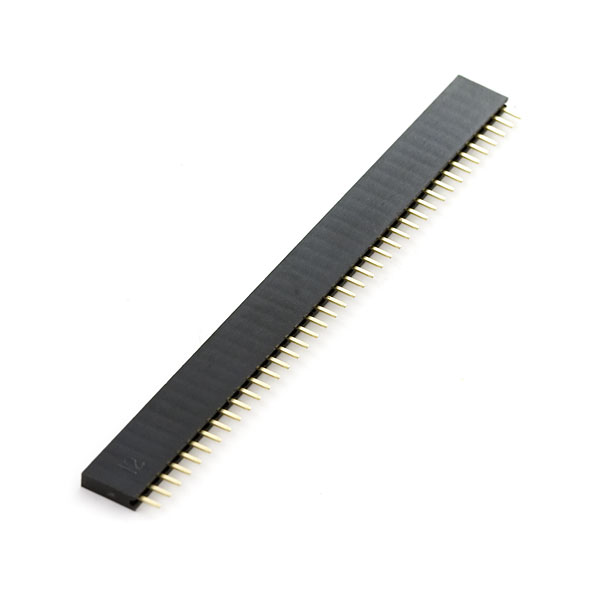
\includegraphics[scale=0.25]{fmbug}
        \caption{Female bug strip}
      \end{figure}
      \newpage
    \item Male bug strip.
    \begin{figure}[!h]
        \centering
        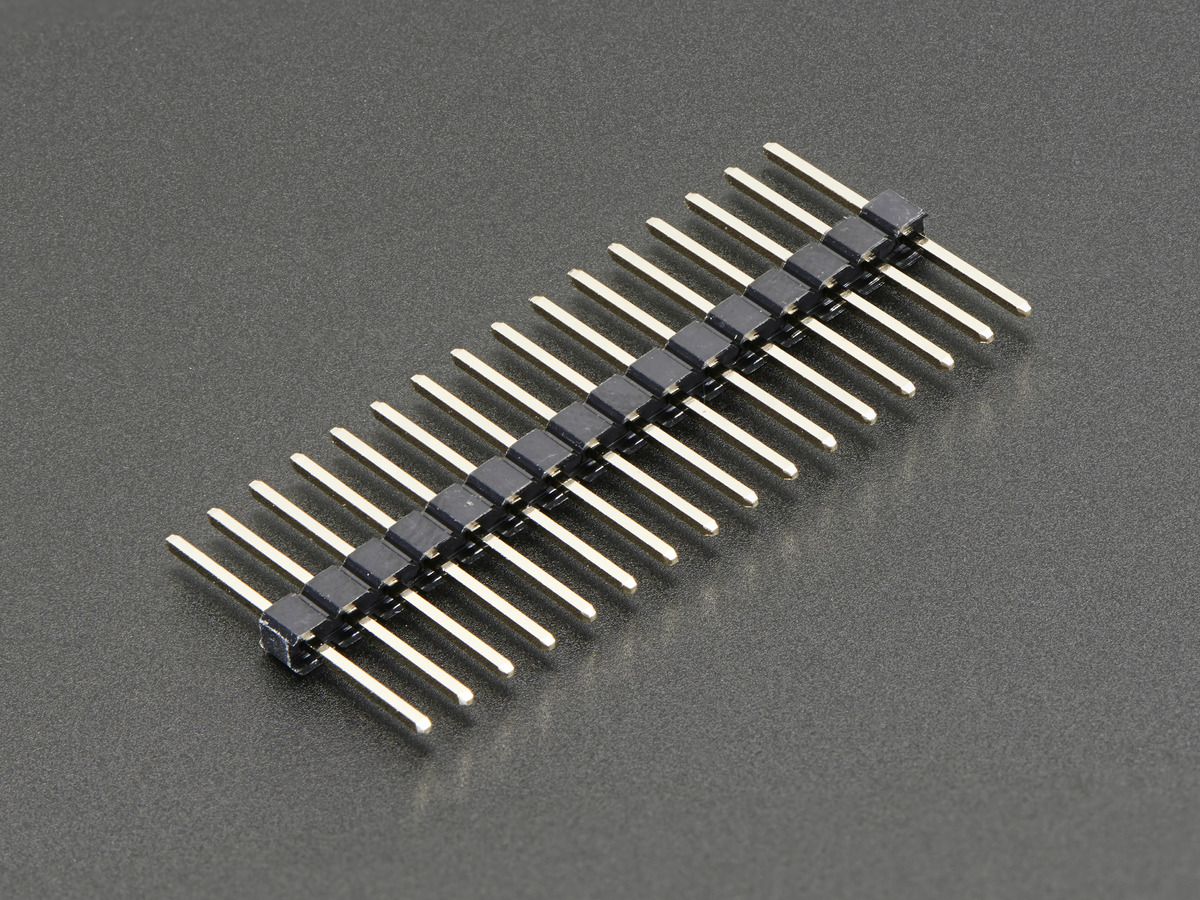
\includegraphics[scale=0.12]{mbug}
        \caption{Male bug strip}
      \end{figure}
    \item Male to Female Jumper Wires.
    \begin{figure}[!h]
        \centering
        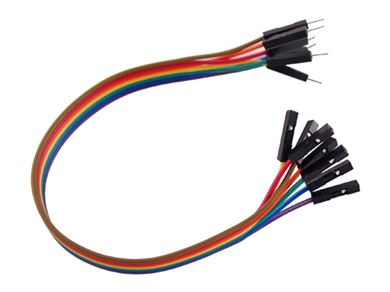
\includegraphics[scale=0.45]{jumper}
        \caption{Jumper Wires}
      \end{figure}\\
    \item Plastic Chassis.\\
     \par
    \begin{figure}[!h]
        \centering
        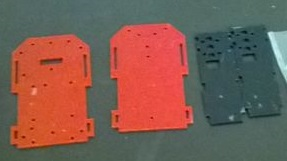
\includegraphics[scale=0.75]{chasis}
        \caption{Chassis}
      \end{figure}
      \newpage
  \end{enumerate}
  \item Hardware used with TIVA board Robot:
   \begin{figure}[!ht]
        \centering
        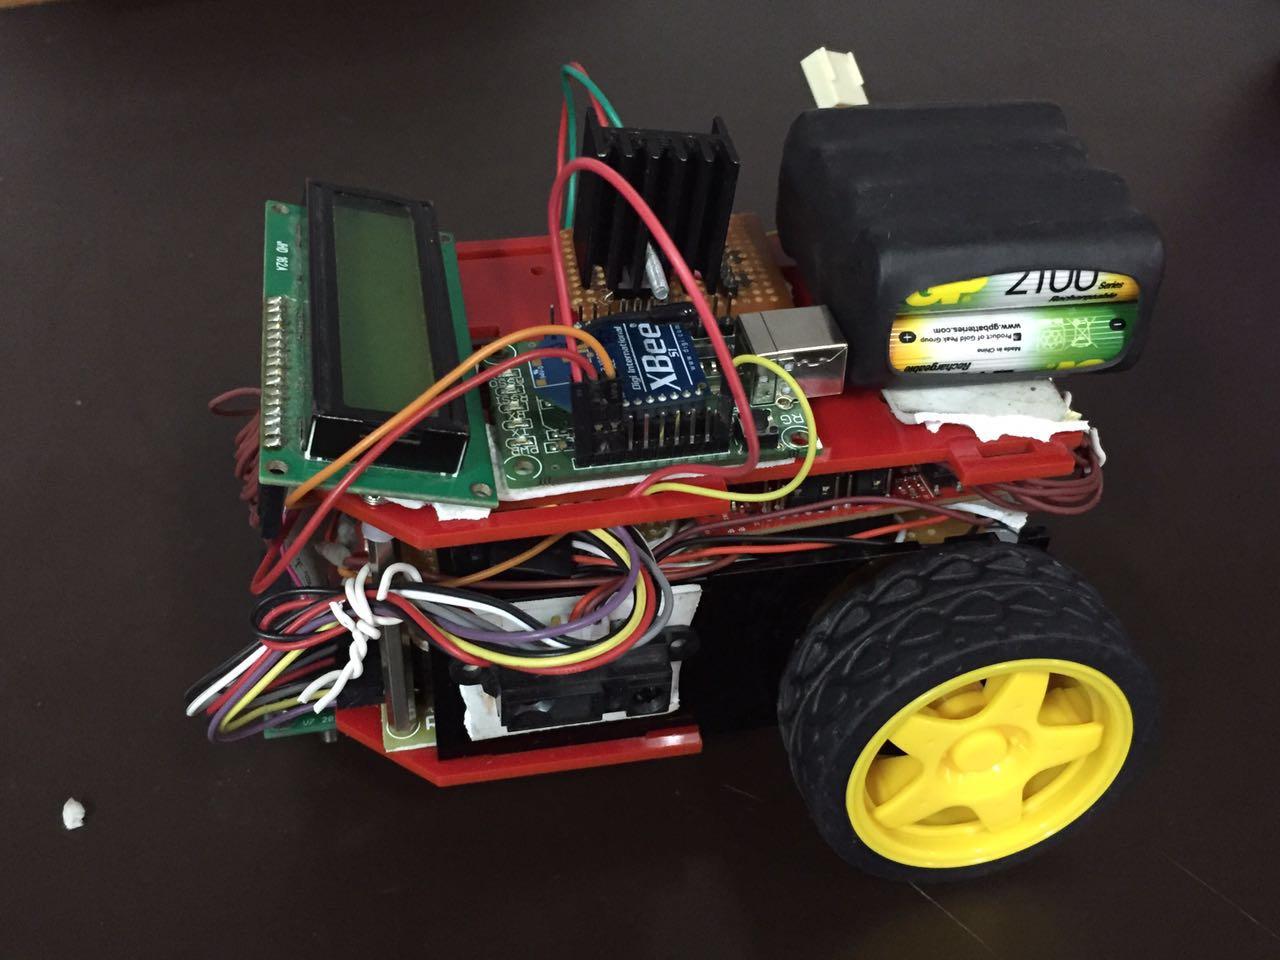
\includegraphics[scale=0.13]{robot}
        \caption{Robot}
      \end{figure}
  \begin{enumerate}
    \item X-Bee Module.
     \begin{figure}[!h]
        \centering
        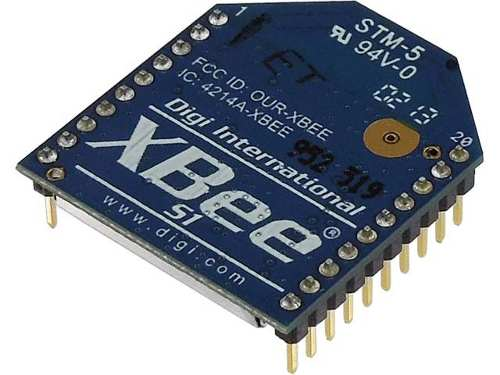
\includegraphics[scale=0.2]{xbee.jpg}
        \caption{xbee module}
      \end{figure}
    \item X-Bee Module and adapter to receive data on a Laptop/PC.
    \begin{figure}[h]
        \centering
        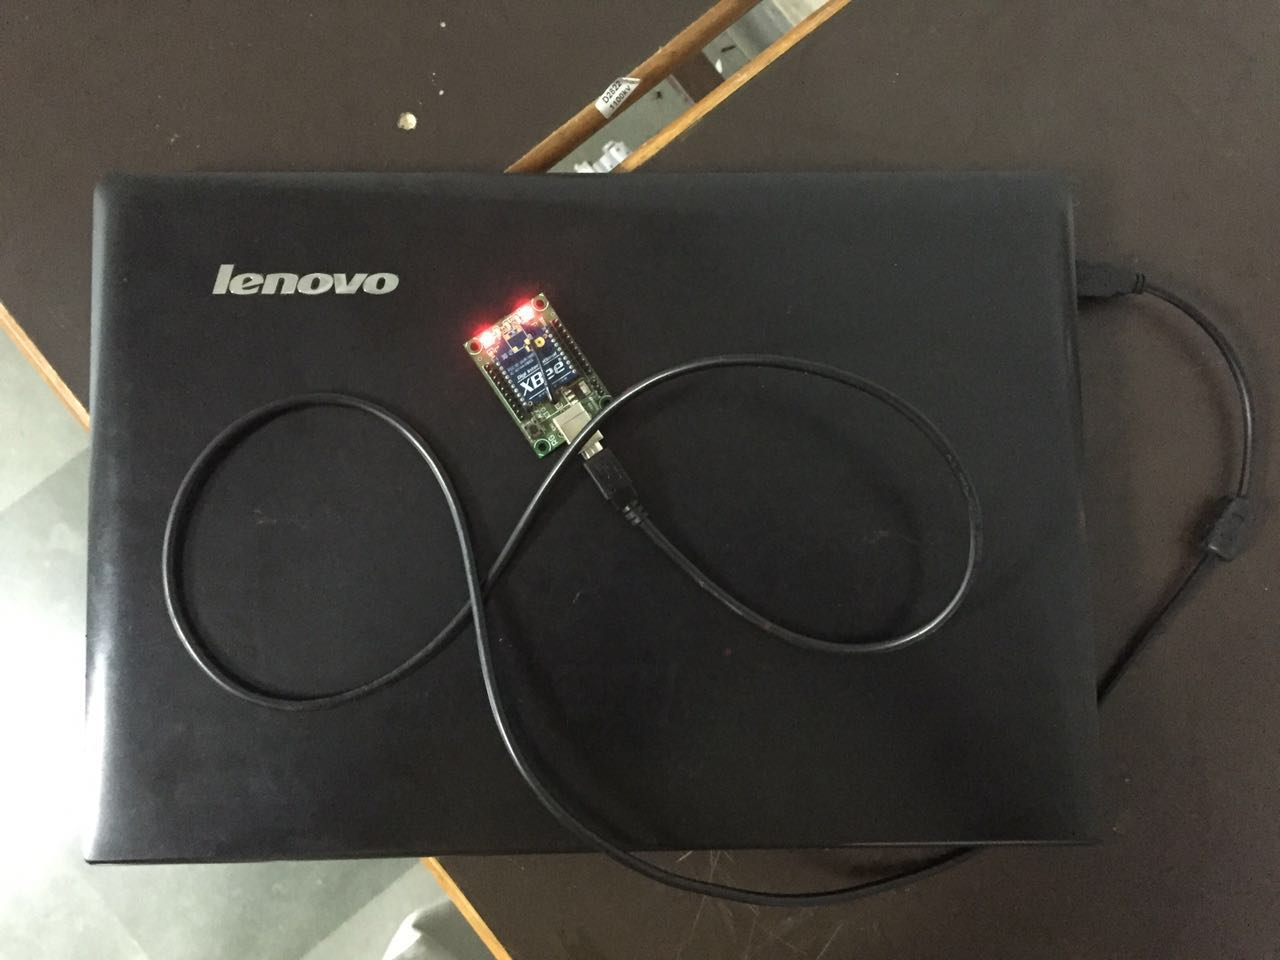
\includegraphics[scale=0.12]{adapter_board}
        \caption{Xbee with adapter connected to laptop}
      \end{figure}
  \end{enumerate}
\end{itemize}
\newpage
\section{Software used}
\begin{itemize}
  \item Atmel Studio 6.0\\
  \href{http://www.atmel.com/forms/software-download.aspx?target=tcm:26-41305}{ Download Here}
  \item XCTU-NG\\
  \href{http://www.digi.com/products/xbee-rf-solutions/xctu-software/xctu}{ Download link}
  \item Serial Terminal\\
  \href{http://www.nex-robotics.com/images/downloads/Terminal\%20Setup.zip}{Download link}
  \item Code Composer Studio v6.1.3\\
  \href{http://www.ti.com/tool/ccstudio}{Download link}


  \item NetBeans IDE 8.1\\
  \href{https://netbeans.org/downloads/}{Download link}
  \item AVR bootloader\\
  \href{http://www.nex-robotics.com/images/downloads/AVR\%20Boot\%20Loader.zip}{Download link}
\end{itemize}
\newpage
\section{Assembly of hardware}
\subsection{Firebird V Robot}
Xbee module is attached with Firebird V robot to collect it's state.
\begin{figure}[h]
        \centering
        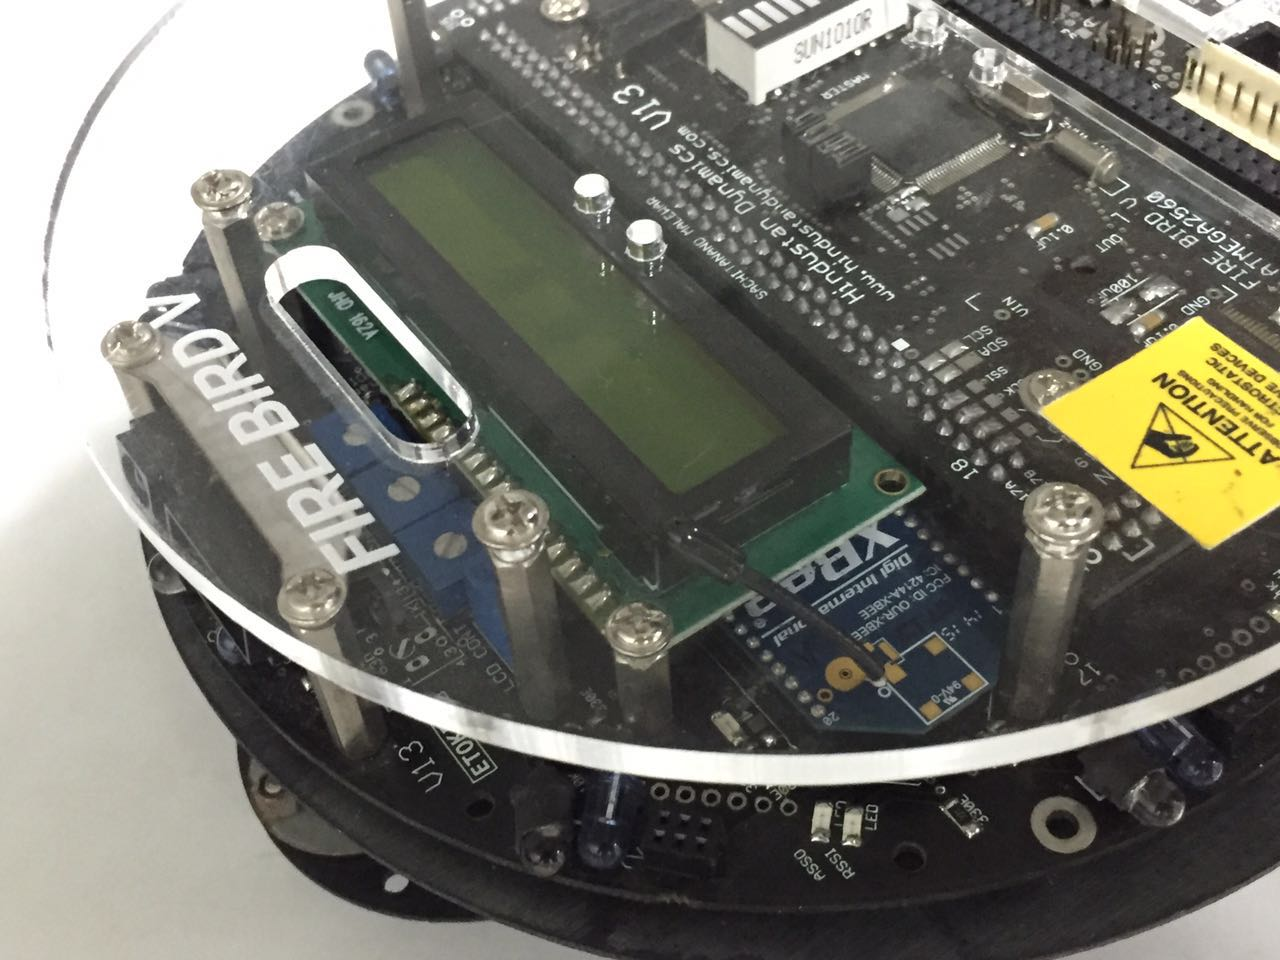
\includegraphics[scale=0.19]{xbee_connected}
        \caption{Xbee connected with firebird V}
      \end{figure}
\subsection{Tiva robot}
Connections of PORT pins of Tiva board with different components:\\
\begin {enumerate}
\item Interfacing of white line sensor
\begin{itemize}
\item PE1  - LEFT   SENSOR
\item PE2  - CENTER SENSOR
\item PE3  - RIGHT  SENSOR
\item GND  - GND
\item VCC  - VCC
\end{itemize}
\item Interfacing of Sharp sensor
\begin{itemize}
\item PE0  - Sharp   SENSOR
\item GND  - GND
\item VCC  - VCC
\end{itemize}
\item Interfacing of Motor Driver IC
\begin{itemize}
\item PE4  - PWM1
\item PA2  - IN1
\item PA3  - IN2
\item GND  - GND
\item VCC  - VCC
\item PE5  - PWM2
\item PA6  - IN3
\item PA7  - IN4
\end{itemize}
\item Interfacing of X-Bee module
\begin{itemize}
\item PC4  - Rx
\item PC5  - Tx
\item GND  - GND
\item VCC  - VCC
\end{itemize}
\item Interfacing of Buzzer
\begin{itemize}
\item PF0  - Signal
\item GND  - GND
\end{itemize}
\item Interfacing of LCD
\begin{itemize}
\item PB0  - DATA 0
\item PB1  - DATA 1
\item PB2  - DATA 2
\item PB3  - DATA 3
\item PB4  - DATA 4
\item PB5  - DATA 5
\item PB6  - DATA 6
\item PB7  - DATA 7
\item GND  - GND
\item VCC  - VCC
\item VEE  - GND
\item VCC  - Led+
\item GND  - Led-
\item PA4  - RS
\item PA5  - RW
\item PC6  - EN
\end{itemize}
\end{enumerate}
\subsection*{Block Diagram}
Basic connections different components of Tiva robot.
\\
\begin{figure}[h]
        \centering
        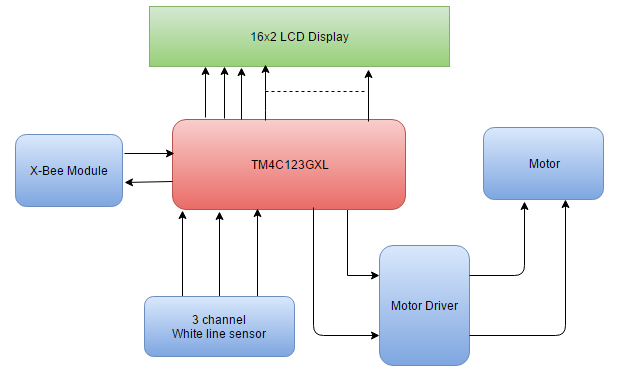
\includegraphics[scale=0.9]{Block}
        \caption{Block diagram of Tiva robot}
      \end{figure}
      \newpage
\subsection{Steps for assembling Tiva robot}
\begin{enumerate}
\item All the components.
\begin{figure}[h]
        \centering
        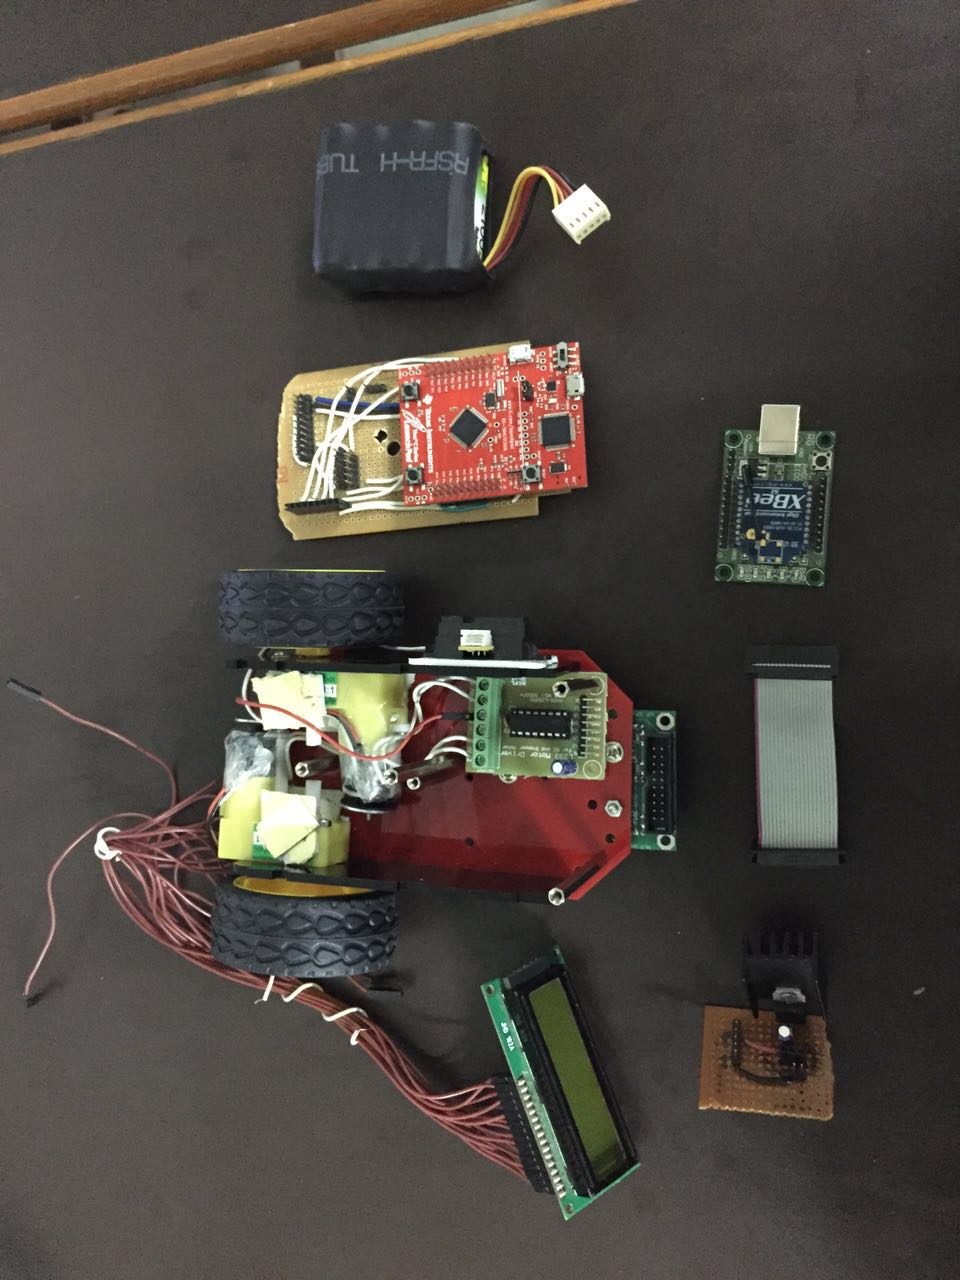
\includegraphics[scale=0.16]{all_components}
        \caption{All the components used to build the bot.}
      \end{figure}
\item Chassis,two dc geared motors \& two wheels are assembled and the wheels are connected with the motor driver IC.
\begin{figure}[h]
        \centering
        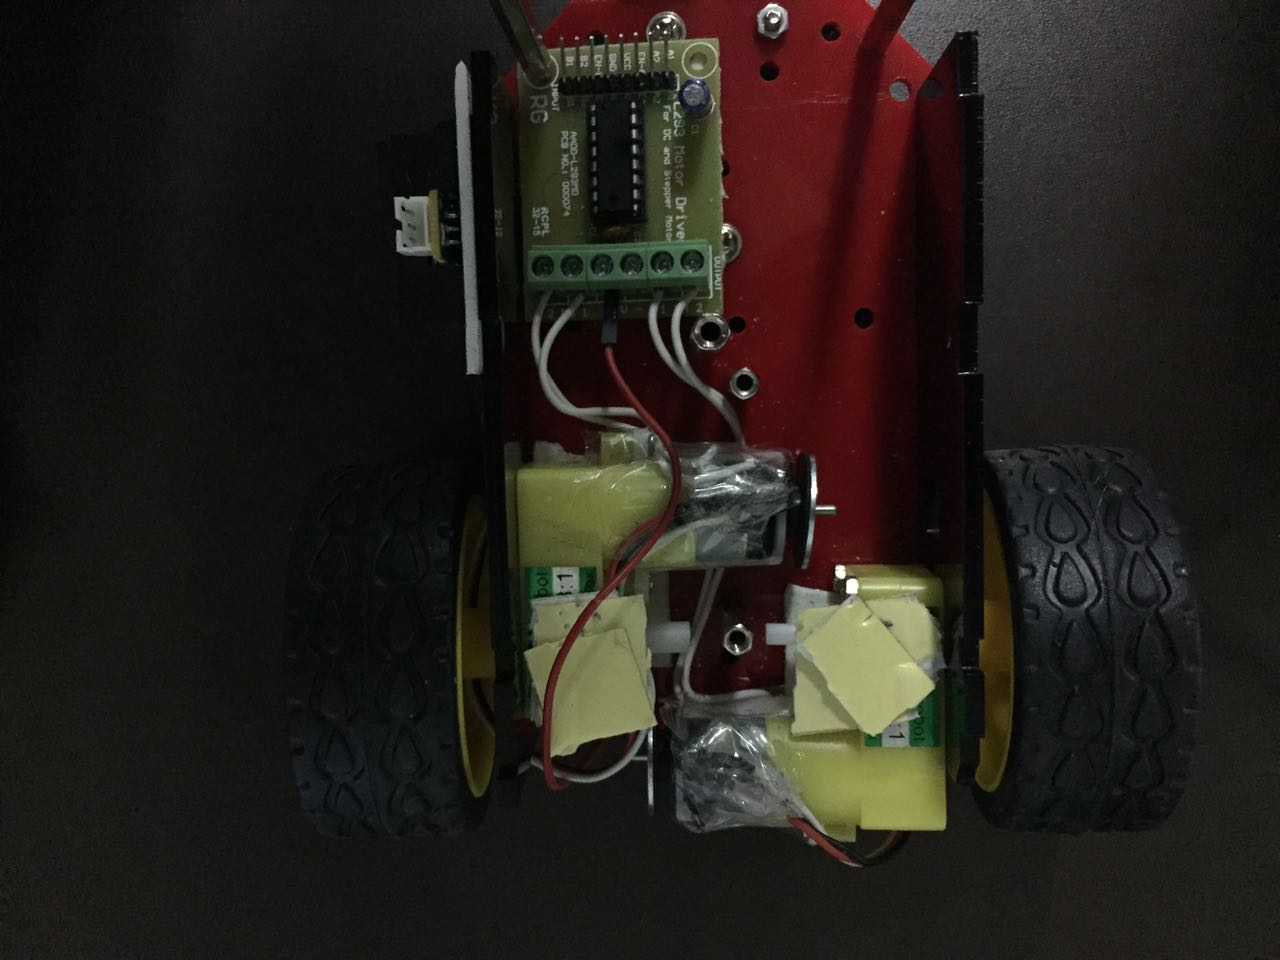
\includegraphics[scale=0.16]{motor_2_ic}
        \caption{Motors and wheels attached to chassis}
      \end{figure}
      \newpage
\item Whiteline sensors and Caster wheel is connected to the chassis.
\begin{figure}[h]
        \centering
        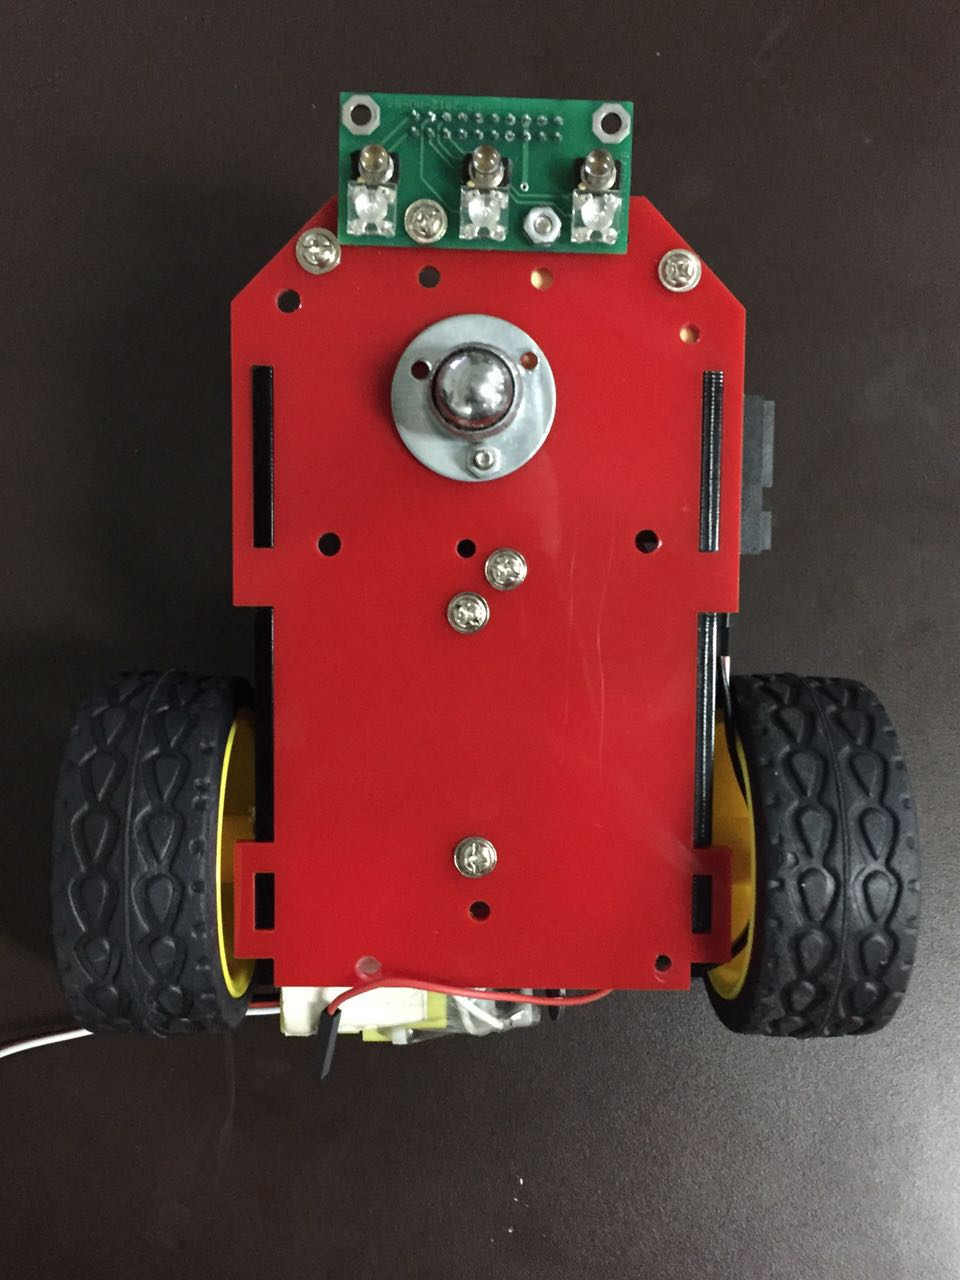
\includegraphics[scale=0.16]{caster_whiteline}
        \caption{Caster Wheel and Whiteline Sensors attached to chassis}
      \end{figure}

\item Sharp Sensor is attached to the chassis.
\begin{figure}[h]
        \centering
        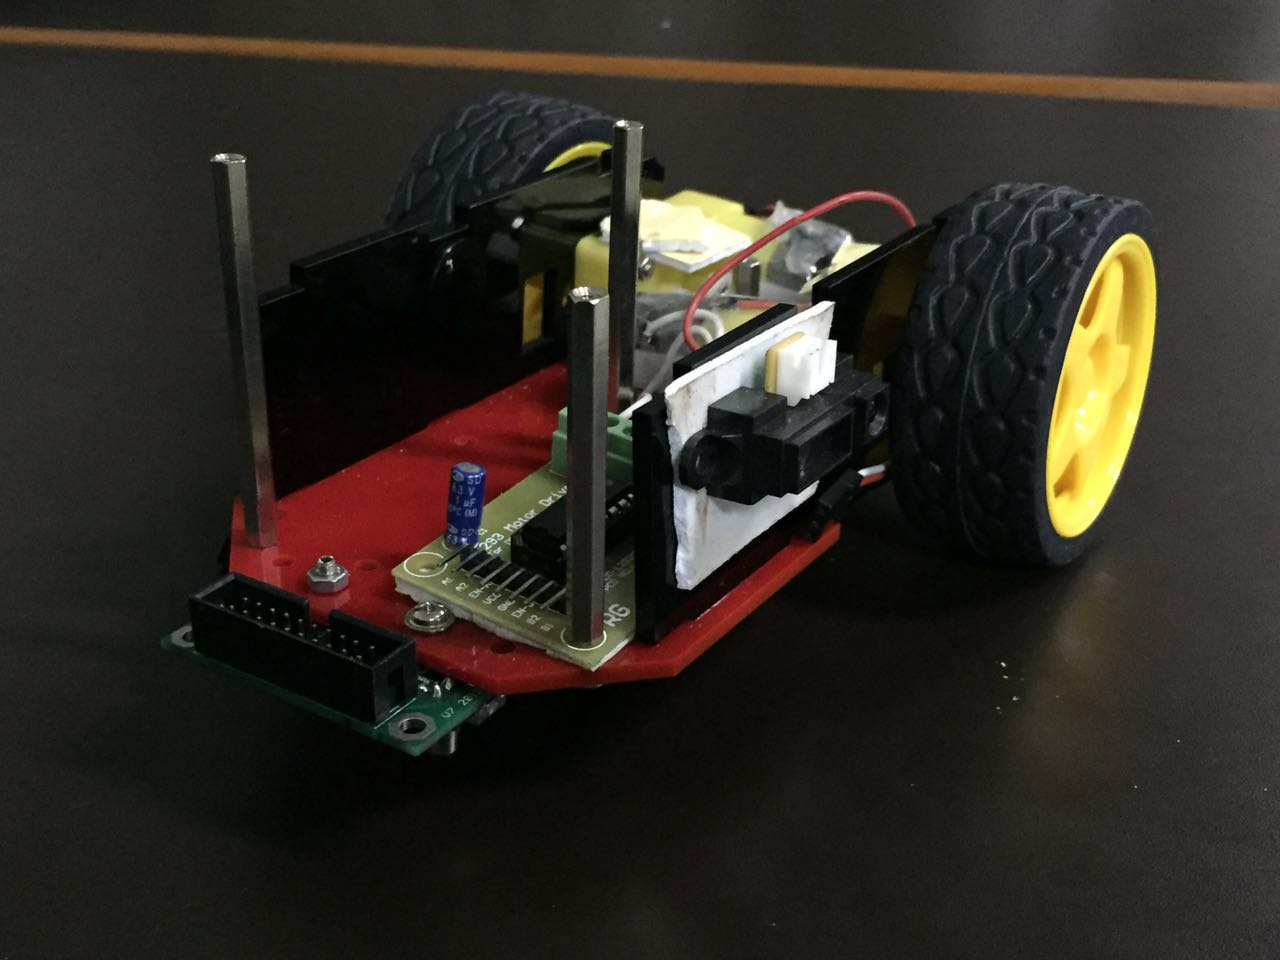
\includegraphics[scale=0.16]{a_sharp}
        \caption{SHARP Sensor attached to chassis}
      \end{figure}
      \newpage

\item Buzzer is attached to the PCB board designed on which TIVA board would fit and attached to the chassis.
\begin{figure}[h]
        \centering
        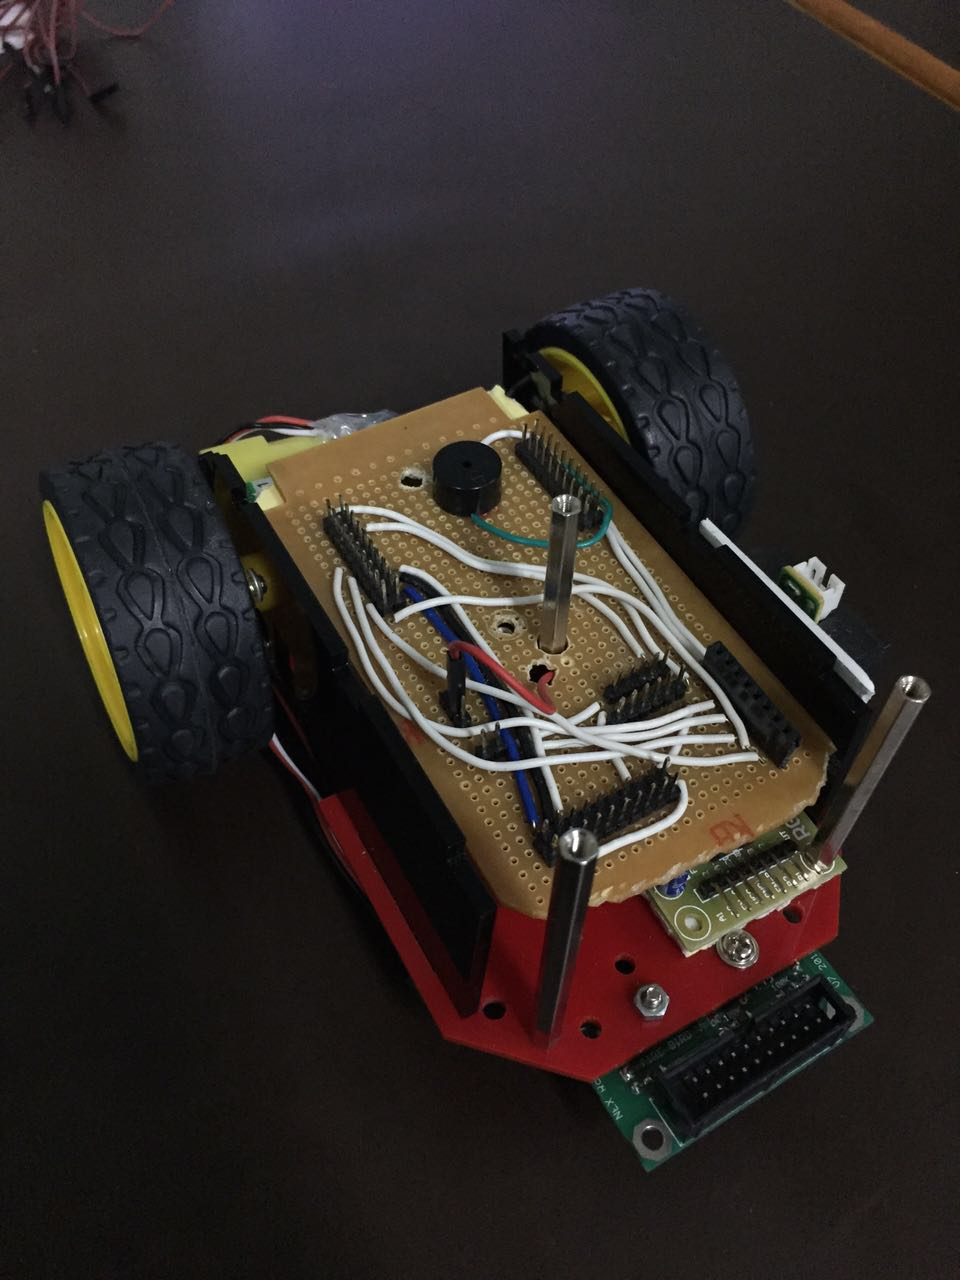
\includegraphics[scale=0.16]{buzzer}
        \caption{Buzzer which would be beneath the TIVA board}
      \end{figure}
\item TIVA board (TM4C123GXL) is attached on the PCB board.
\begin{figure}[h]
        \centering
        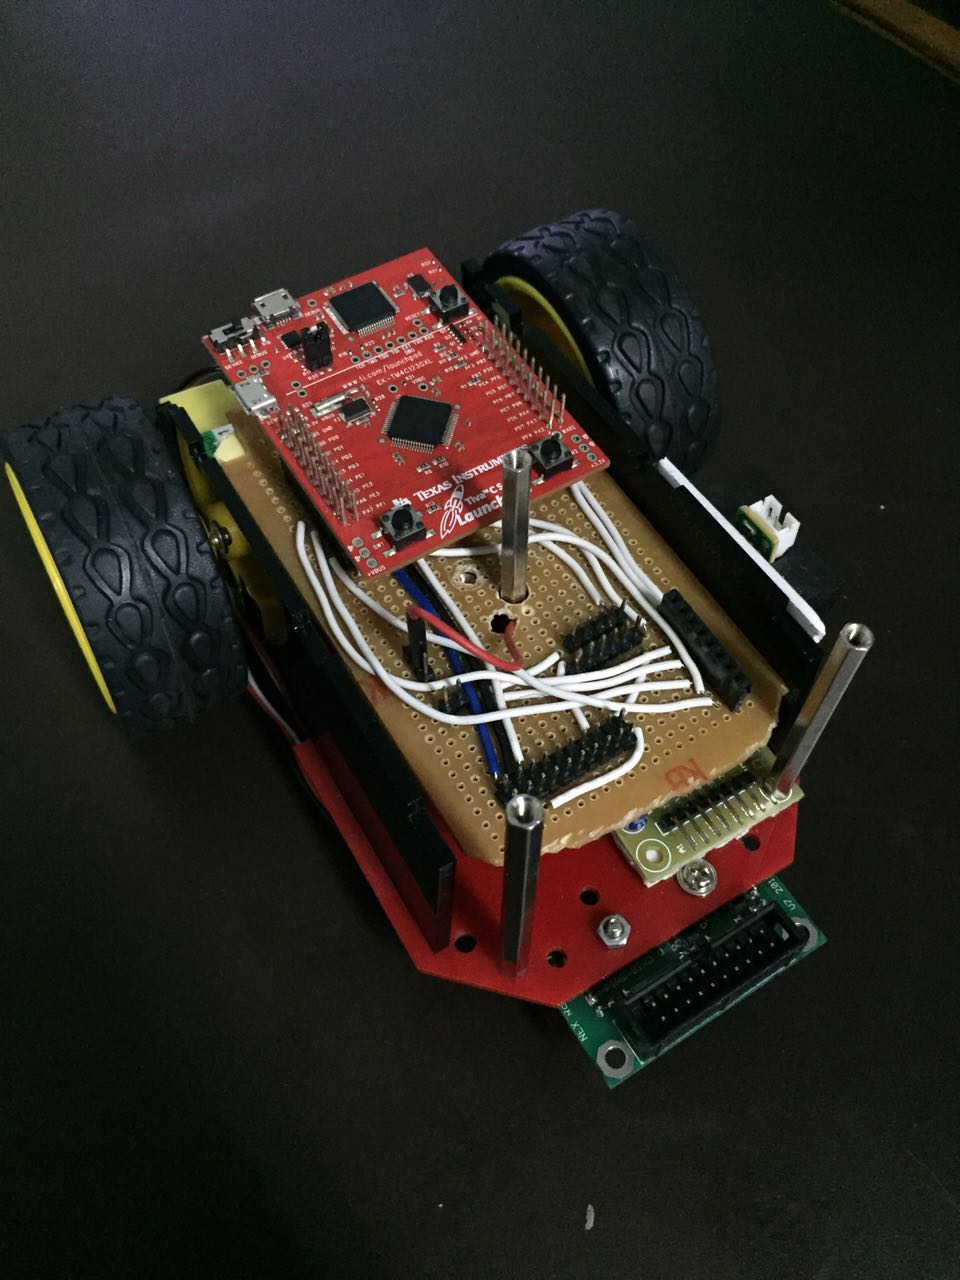
\includegraphics[scale=0.13]{tiva_attatched}
        \caption{TIVA board fitted}
      \end{figure}
    \newpage

\item Whiteline Sensors are connected using the 20 pin connector.
\begin{figure}[h]
        \centering
        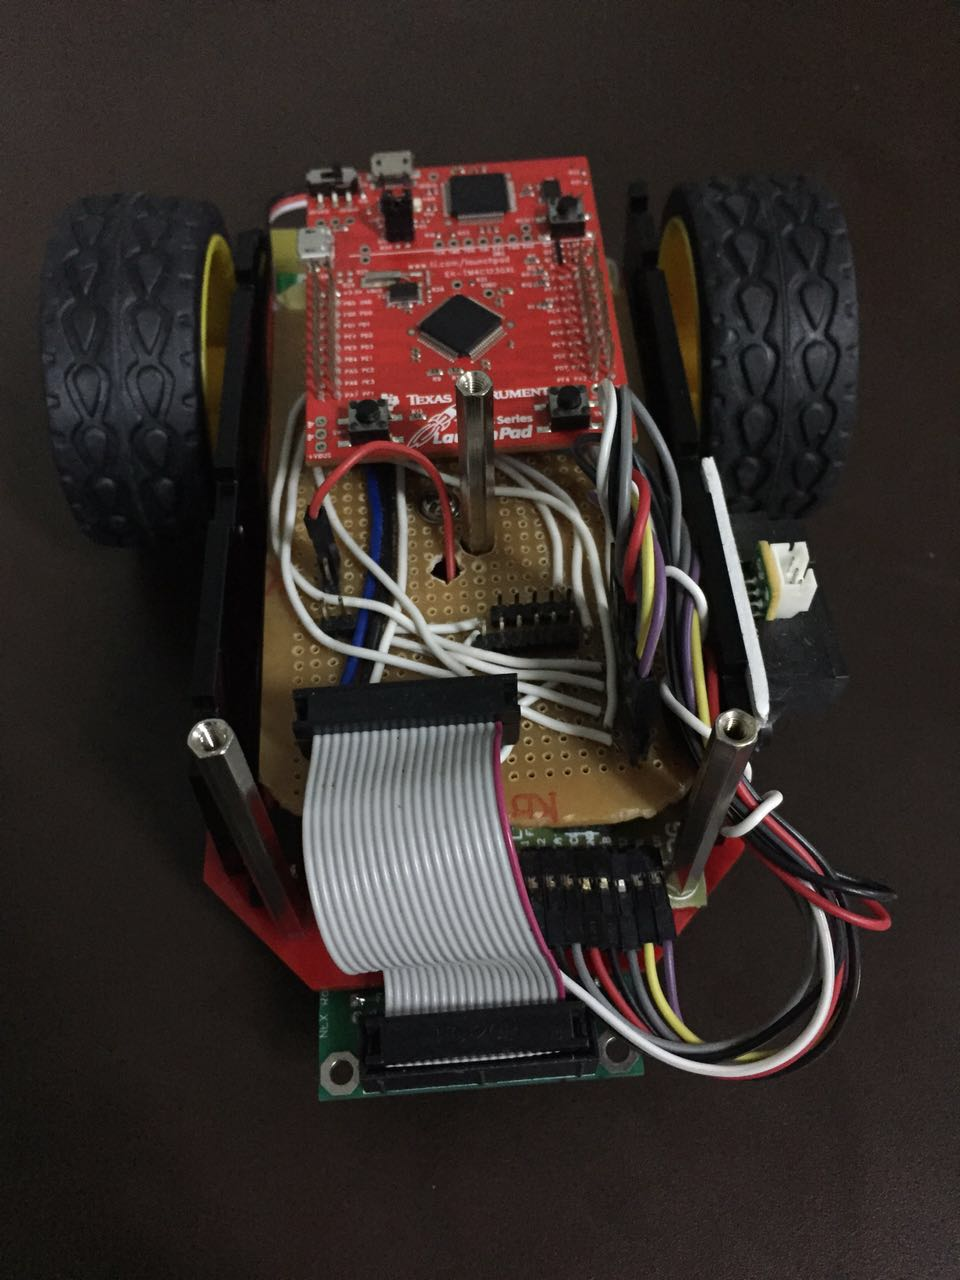
\includegraphics[scale=0.16]{wh_attatched}
        \caption{Whiteline Sensors are now connected to the TIVA board.}
      \end{figure}

\item SHARP Sensor and Motor Driver IC are connected to the TIVA board.
\begin{figure}[h]
        \centering
        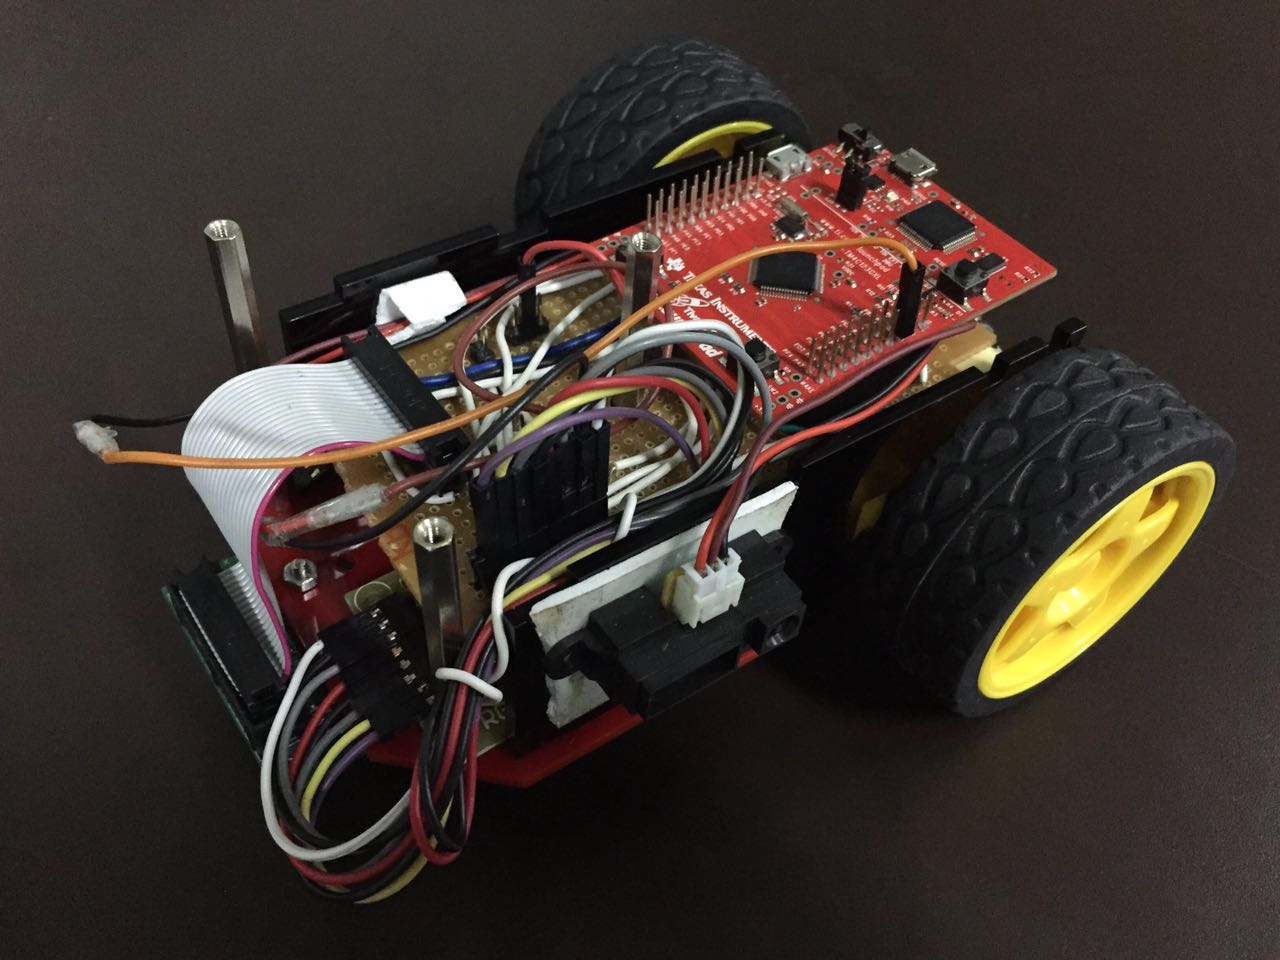
\includegraphics[scale=0.16]{all_connected}
        \caption{SHARP Sensor and Motor Driver IC are now connected to the TIVA board.}
      \end{figure}
      \newpage

\item LCD is now connected to the TIVA board.
\begin{figure}[h]
        \centering
        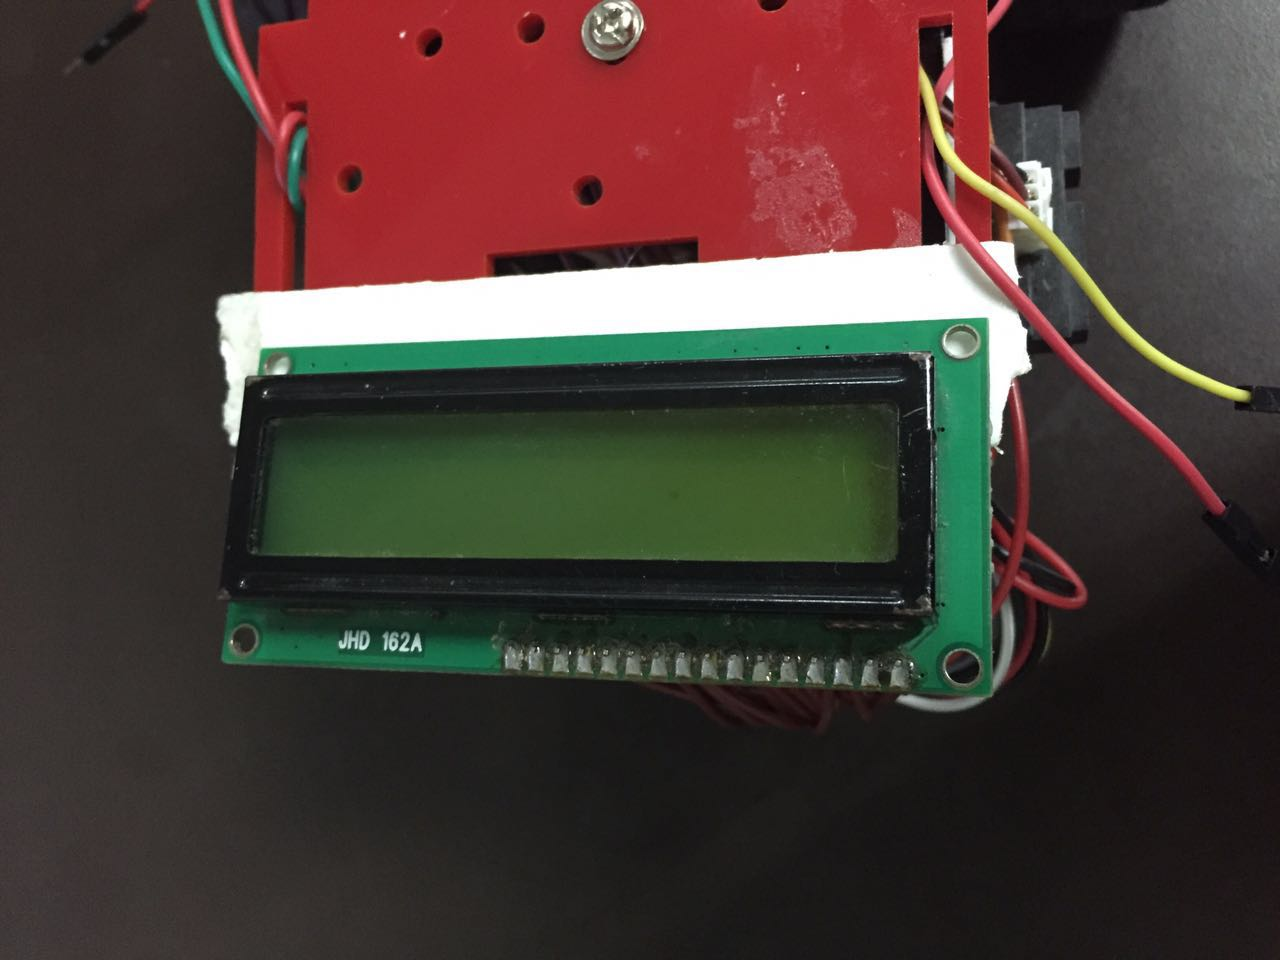
\includegraphics[scale=0.16]{lcd_a}
        \caption{LCD after being attached to the bot.}
      \end{figure}

\item X-Bee is now connected to the TIVA board.
\begin{figure}[h]
        \centering
        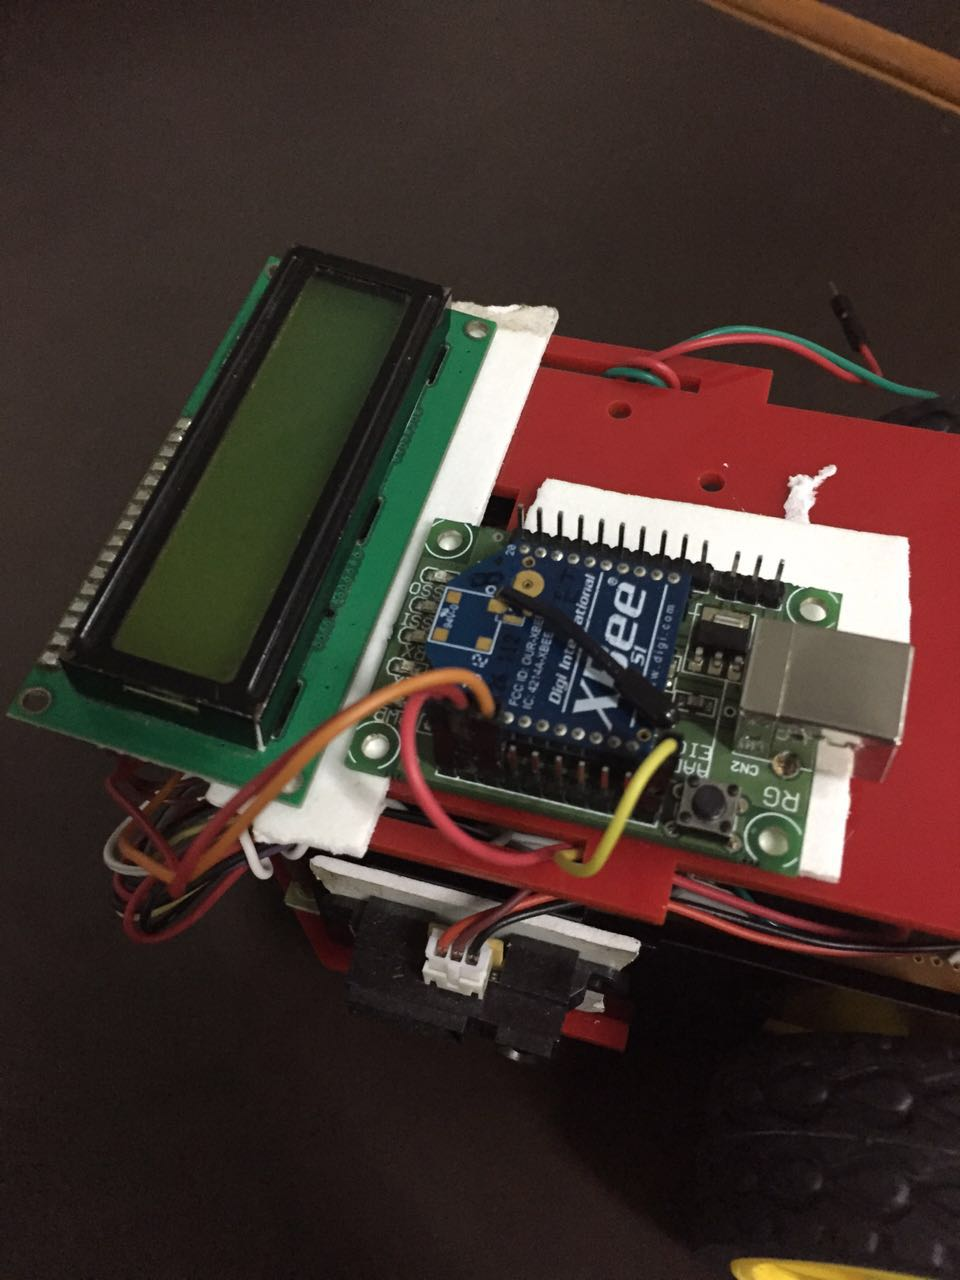
\includegraphics[scale=0.16]{xbee_a}
        \caption{X-bee after being attached to the bot.}
      \end{figure}
      \newpage

\item Voltade Regulator Circuit and Battery are now connected to the TIVA board.
\begin{figure}[h]
        \centering
        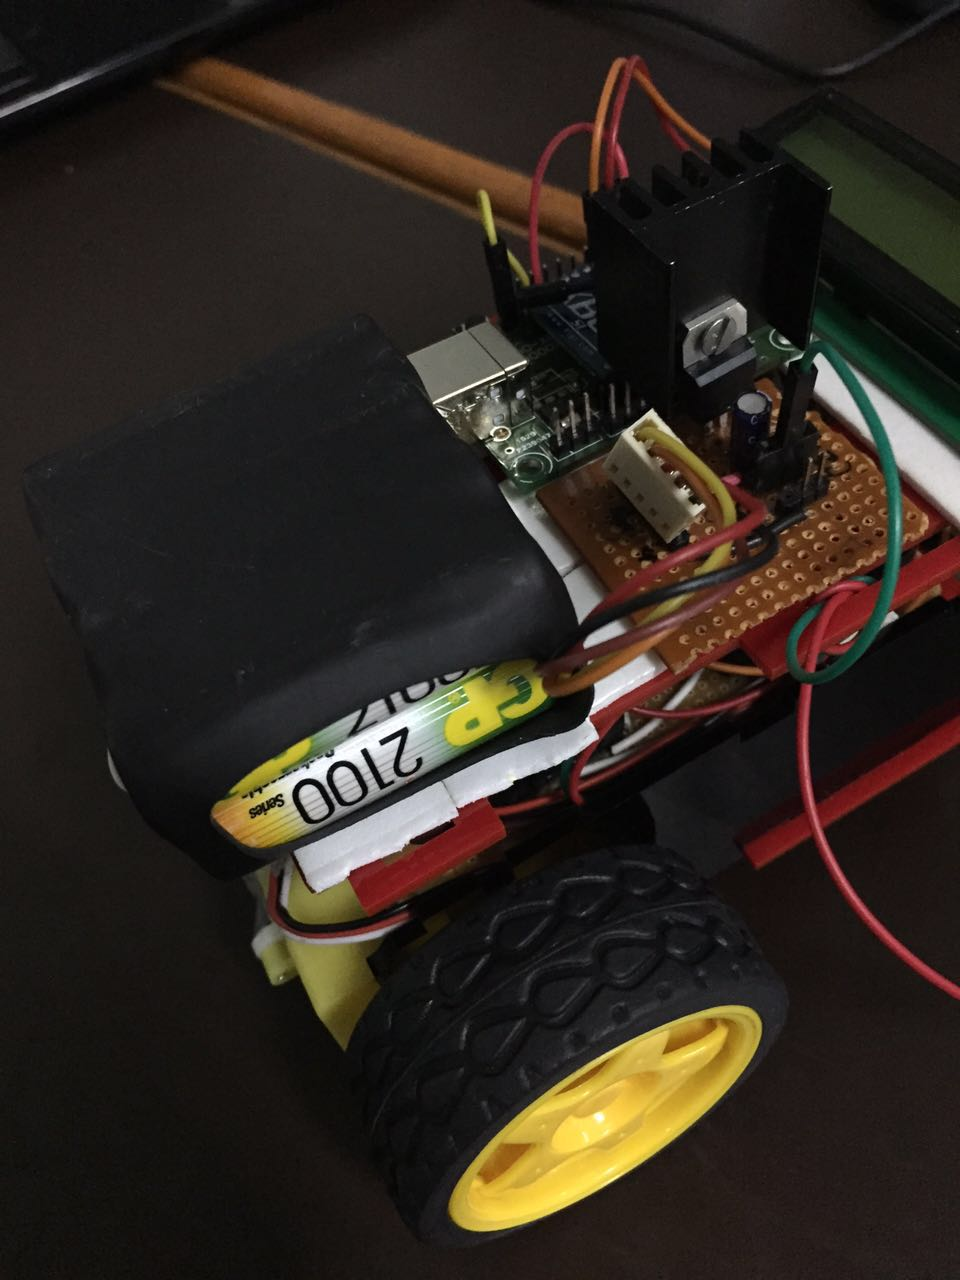
\includegraphics[scale=0.16]{battery_a}
        \caption{Power can now be supplied to the bot.}
      \end{figure}

\item Finally the Bot is Ready for use.
\begin{figure}[h]
        \centering
        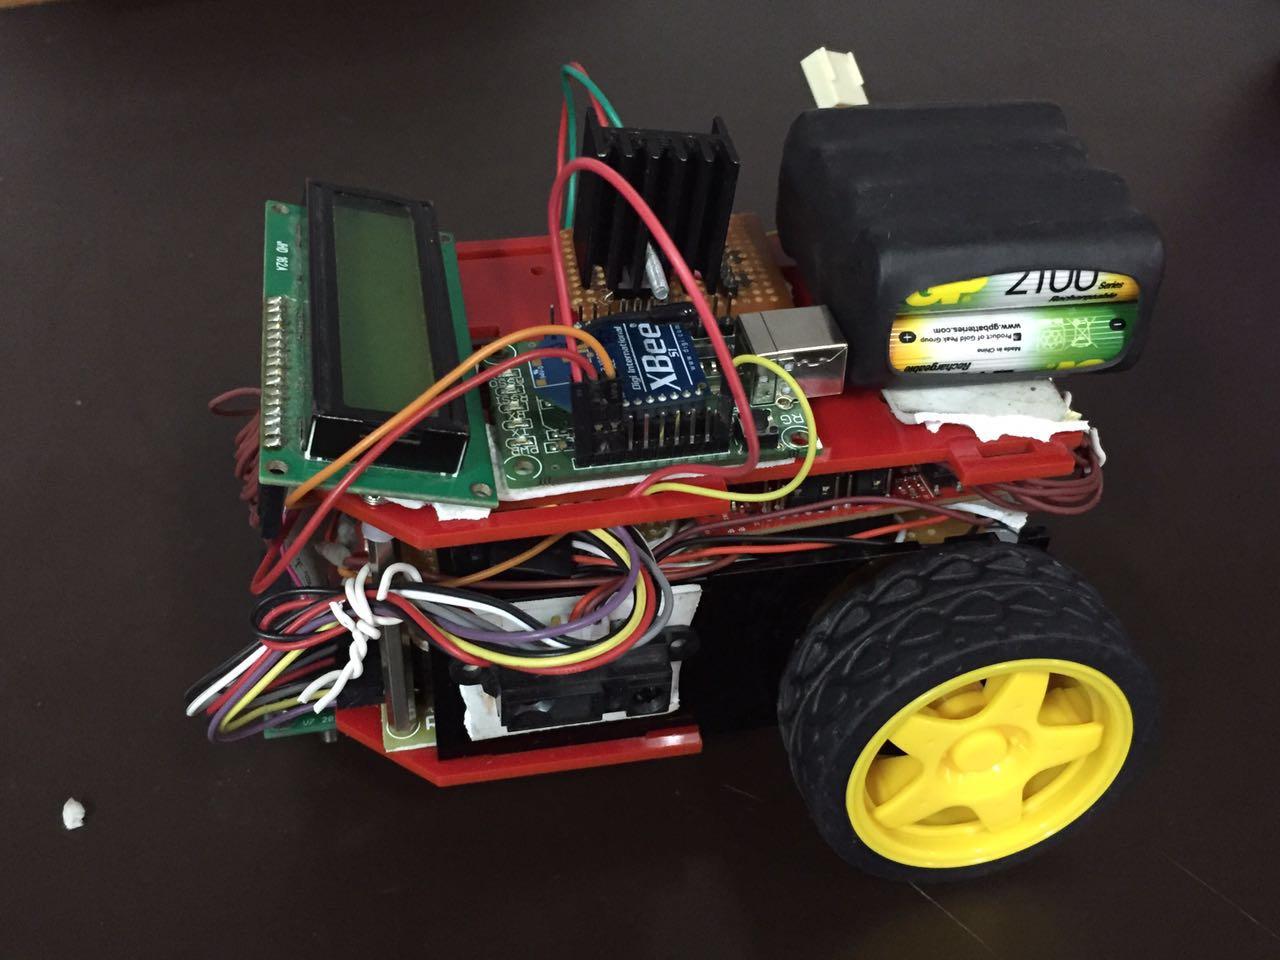
\includegraphics[scale=0.16]{robot}
        \caption{TIVA BOT.}
      \end{figure}
    \newpage
\end{enumerate}

\newpage
\section{Software and Code}
\href{https://github.com/eYSIP-2016/Robot_State_Collector/tree/master/code}{Github link} for the repository of code
\subsection{Sate Collection code For Firebird V Robot}
We are using Timer4 to generate an interrupt after 0.5s. Using this interrupt we can send the present values of the sensors to the GUI.\\
    Our code is entirely inside the provided header file. A simple function call starts the State Collection.

\subsection{Sate Collection code For TIVA Robot}
    We are using Timer0A to generate an interrupt after 0.5s. Using this interrupt we can send the present values of the sensors to the GUI.\\
    Our code is entirely inside the provided header file. A simple function call starts the State Collection.

\subsection{GUI}

The GUI is capable of reading the incoming data on the X-Bee module. The data is stored and on a press of a button it gets encrypted using a symmetric key algorithm , the key of this symmetric key algorithm is encrypted using the public key provided to the user. At the end the encrypted data can be sent to the server if the user wishes.

\newpage

\section{Use and Demo}

\subsection{Steps for merging the State Collection Code with User's Code for Firebird V}
\begin{enumerate}

\item include "common\_header.h" in User' Code
\item include "state\_collect.h" in User' Code

\item In main after initialising all the devices call the function  "\_init\_devices()"

\end{enumerate}

State Collection will now take place with the User's Code.\\

NOTE : The files included above should be present inside the same folder as that of the User's code.

\subsection{Steps for merging the State Collection Code with User's Code for TIVA bot}
\begin{enumerate}

\item include "common\_header.h" in User' Code
\item include "collect.c in User' Code
\item include "sensor.c in User' Code
\item In main call the function  "start\_collection()" and "sensor\_pin\_config".

\end{enumerate}

State Collection will now take place with the User's Code.\\

NOTE : The files included above should be present inside the same folder as that of the User's code.

\subsection{Steps for using the GUI}
\begin{enumerate}

\item Login with the credentials provided.
\item Make sure that the X-Bee adapter is connected to the laptop.
\item Click on the "Search for available COM ports " button.
\item From the Drop Down Menu select the COM port on which the X-Bee adapter is connected. Selecting the COM port would establish a connection with the X-Bee and the "Not connected" would change to "Connected".
\item After the run is complete Click on "End of Run" button to indicate the end of the robot's task.
\item To send the data to the server click on "Connect to the Server" button.
\item To disconnect from the COM port press the "Disconnect" button.

\end{enumerate}

\newpage

\section{Future Work}

\begin{enumerate}

\item LCD data can be collected.
\item Server Side Code can be improved such that it shouldn't have to be restarted after each run.
\item Position encoders can be configured with the TIVA Bot.

\end{enumerate}

\newpage

\section{Bug report and Challenges}

\subsection{Bugs:}


\begin{enumerate}

\item X-Bee doesn't run at baud rate of 115200 on Firebird V.
\item X-Bee doesn't run at baud rate of 9600 on TIVA bot.
\item If we change the frequency of the system clock on TIVA bot the X-Bee doesn't work.
\item Java code at server side stops after each run.
\item If we have to collect data of the position encoders then it has to be done with the interrupt used by the user and hence we have to change the user's code a bit.
\item The server side code hasn't been tested with multiple clients.
\item The server would give an error if the user logs in and closes the GUI without sending the data.
\item We don't know what would happen if connection between the client and the server is lost while transmitting the data.
\item There would be a loss of data if the user presses the Disconnect button while the GUI is collecting the State data.
\item On TIVA board no formula for conversion of digital values of SHARP sensor to actual distance has been used as TIVA board has a 12 bit ADC channel and all the formulas we found were meant for 8 bit ADC channels.

\end{enumerate}

\subsection{Challenges:}

\begin{enumerate}

\item Storing the Data efficiently on the bot's memory -- This was avoided by sending the data using a X-Bee module.
\item We were first transmitting the data as soon as it was read. This caused a problem as the earlier data was not sent and the new data arrived which caused them to overlap and hence resulted in loss of information -- This was solved by waiting for the previous data to be sent first and then sending the new data.
\item Encryption without using any padding as the data size was not a multiple of 16 bytes and hence the AES encryption algorithm would fail -- This was solved by using a padding which ensures that the data is always a multiple of 16 bytes.
\item Sending the data in a integer format using X-Bee module -- This was solved by digitising the integer and then sending it.
\item Sending the data in a string form over Java Sockets -- This was solved by converting the strings to byte arrays and then sending them.
\item Power when provided directly at VBUS of the TM4C123GXL it would cause the robot to restart -- This problem disappeared after 2 days.
\item Motor Driver IC would not run from the 5V coming from the TIVA board -- This problem disappeared during testing.
\item The PIN PF0 was locked and we were unaware of this fact and tried using this port like any other pin -- After a lot of research on the web we found how to unlock the PINS.

\end{enumerate}


\begin{thebibliography}{li}

yet to be done. :P

\end{thebibliography}


\end{document}

